\documentclass[a4paper,12pt]{article}
\usepackage[frenchb]{babel}
\usepackage[utf8]{inputenc}
\usepackage[T1]{fontenc} 
\usepackage{float}
\usepackage{graphicx}
\usepackage{geometry}
\usepackage{amsmath}
\usepackage{tikz}
\usepackage{pdfpages}
\usetikzlibrary{trees}

\graphicspath{{graphics}{../images/}}

\geometry{margin=2cm}

\begin{document}
\begin{center}
\begin{tabular*}{\textwidth}{l @{\extracolsep{\fill}} r}

  
\includegraphics [width=40mm]{ENSEIRB-MATMECA.jpg} &
  \raisebox{0.75\height}
           {
\includegraphics [width=40mm]{logo-LaBRI-couleur.jpg}}

\end{tabular*}

\vspace{\stretch{1}}

\textsc{\Huge Des bots pour NetHack}\\[0.5cm]
\rule{0.4\textwidth}{1pt}

\vspace{\stretch{1}}

\begin{center}
  
  \begin{flushleft}
    \large
    \emph{Auteurs :}\\
    \begin{itemize}
    \item Benoît Ruelle
    \item David Bitonneau
    \item Ludovic Hofer
    \end{itemize}
  \end{flushleft}
  
  
  \begin{flushright}
    \large
    \emph{Responsables :}\\
    Pédagogique - M.~Renault\\
    Client - M.~Le Borgne\\
  \end{flushright}
\end{center}

\vspace{\stretch{1}}
                  
{\large Deuxième année, filière informatique}

~

{\large 16 octobre 2012 - 29 mars 2013}\\
                  
\end{center}
\thispagestyle{empty}
\pagebreak

\tableofcontents
\pagebreak

\section{Introduction}

NetHack est un rogue-like (jeu inspiré du jeu vidéo \emph{Rogue} - 1980)
sorti en 1987. Le joueur incarne un aventurier chargé de récupérer une
amulette dans un donjon peuplé de monstres.
Les enjeux du projet sont multiples : il s'agit tout d'abord de proposer une
base au développement de bots pour NetHack puis, dans un second temps, de
fournir des méthodes d'évaluation de ces bots. Pour cela la modification du code
de NetHack est nécessaire afin d'établir un moyen de communication entre le
noyau du jeu et les bots ; NetHack étant un jeu écrit en C et sous licence
libre, son code source est disponibles et modifiable. Afin d'évaluer les bots
différents outils de benchmarking ont été mis en place ; ces outils reposent
sur la récupération de données et le stockage de celles-ci afin d'effectuer
des statistiques et produire des graphiques de comparaison.
Par ailleurs, un certain nombre de simplifications du jeu original ont été
opérées dans le but de faciliter le développement des bots et permettre
l'étude de problèmes plus spécifiques.  

Le projet consiste donc en un ensemble de modifications du code du jeu
original, d'ajout d'outils, de fonctionnalités et d'études théorique.

\subsection*{Description du jeu}
-> Ensembles de donjons, de niveau, de cases, etc.
-> monstres, pièges, faims, quêtes, objets, personnages, etc.

\section{Environnement de création de bots}

\subsection{Prototypage}

NetHack propose, dès sa première version, une interface ASCII qui représente un donjon sous la forme suivante:

\begin{verbatim}
                                           Weapons
                                           a - a blessed +1 mace (weapon in hand)
                                           Armor
   -------        ------------             b - a +0 robe (being worn)
   .......         ........>.|             c - a +0 small shield (being worn)
   |.....|        |..........|             Comestibles
   |......#       |@.........|             e - a clove of garlic
   |<....|#       |..........+             f - a sprig of wolfsbane
   |.....|#       -.---- -----             Spellbooks
   -------############                     g - a spellbook of create monster
         #############                     h - a spellbook of detect food
         # #        ##                     Potions
                                           d - 4 potions of holy water
                      .                    Tools
                      ..                   i - an oil lamp
                       ..                  (end) 
                       ...
                       ...
                       ----

JohnDoe the Aspirant          St:11 Dx:14 Co:13 In:11 Wi:15 Ch:11  Chaotic
Dlvl:1  $:0  HP:14(14) Pw:8(8) AC:7  Exp:1
\end{verbatim}

Le \verb!@! désigne le joueur, les caractères \verb!|! et \verb!-! sont des murs, les \verb!#! des couloirs, un \verb!+! symbolise une porte, etc.


\subsubsection*{Séquences d'échappement ANSI}

Cette interface fonctionne à l'aide de caractères d'échappement normalisés \footnote{http://www.inwap.com/pdp10/ansicode.txt} permettant de contrôler la position du curseur dans un terminal et d'afficher des caractères à l'endroit souhaité. Par exemple, une séquence '\verb![46;50H|...+#!' affichera la chaîne de caractères '\verb!|...+#!' en commençant à la ligne 46, colonne 50. Il est alors facile de reconstituer une carte envoyée par le jeu: le '\verb!|!' est aux coordonnées (46, 50), le '\verb!+!' est situé à (46, 54), etc.
	
	Le projet TAEB (Tactical Amulet Extraction Bot) \footnote{https://github.com/sartak/TAEB} utilise ce principe pour reconstituer la carte à l'aide d'un module sachant interpréter ces séquences de caractères \footnote{https://metacpan.org/module/Term::VT102}. Une première approche fut donc de copier ce procédé.


\subsubsection*{Pseudo-terminal}

Pour empêcher certaines formes de tricheries, NetHack procède à quelques vérifications pour s'assurer qu'il est bien lancé depuis un terminal, ce qui empêche les redirections de son entrée/sortie. Les quelques lignes de code responsables peuvent être désactivées sans conséquence notable sur le reste du jeu mais cela nécessite de modifier le code original. Pour rediriger à la fois l'entrée et la sortie du jeu sans modifier le jeu, il est nécessaire de 'tromper' NetHack à l'aide d'un pseudo terminal.

Un pseudo terminal (pty) est une paire de pseudo périphériques dont l'un est appelé 'maître' et l'autre 'esclave'. Le maître est utilisé comme un terminal standard sur lequel on peut écrire ou lire du texte. L'esclave communique avec l'application et sert simplement de rapporteur entre la partie 'maître' et NetHack. Ainsi, le jeu est satisfait puisqu'il est lancé depuis un terminal et il peut maintenant être contrôlé depuis la partie 'master' du pty sur laquelle on souhaite brancher un bot \footnote{Plus de détails avec la page de manuel pty(7)}.


\subsubsection*{Décomposition de l'affichage}

Lorsqu'il est lancé depuis un terminal, l'interface ASCII détecte le nombre de lignes et de colonnes disponibles afin de faire des défilements ou des superpositions de menus lorsque nécessaire \footnote{voir termcap}. Cela pose problème avec la méthode consistant à interpréter les séquences d'échappement car il faut être capable détecter lorsque deux éléments se chevauchent.

\begin{figure}[H]
	\caption{Exemple d'un menu recouvrant une partie de la carte}
	\begin{verbatim}
                                     Weapons
                                     a - a blessed +1 mace (weapon in hand)
             ------                  i - a crude bow
             |...[|                  Armor
 -------     |..<..###############`  b - a +0 robe (being worn)
 |......-    .....|       ---------- c - a +0 small shield (being worn)
 |           -.----      #.........| Comestibles
              ##       ###|........| e - a clove of garlic
               #       #  |........| f - a sprig of wolfsbane
               ###   ###  |........| Spellbooks
                 #   #    |........| g - a spellbook of detect food
                 ### #    |........| h - a spellbook of clairvoyance
                ?  # #    --.------- Potions
               ----.-#      ###@#### d - 4 potions of holy water
               |....|#               j - a blessed black potion
               |....|#               (end) 
               +.....#                         |..... ..$|
               |....|                          |.........|
               ------                          |.........|
                                               -----------

JohnDoe the Aspirant          St:10 Dx:14 Co:13 In:9 Wi:18 Ch:11  Chaotic
Dlvl:1  $:0  HP:14(14) Pw:7(7) AC:7  Exp:1
	\end{verbatim}
\end{figure}

Une façon de supprimer cette difficulté est de tromper une nouvelle fois NetHack en manipulant la taille effective du pseudo terminal qui n'est en rien liée à sa taille réelle à l'écran. Avec une taille assez grande, il n'y a jamais de chevauchement.

Nous pouvons ainsi séparer l'écran comme suit en forçant une taille de 24 lignes par 160 colonnes :

\begin{verbatim}
               Messages line ................ --more--
               ----------------------------------------
               |                  |                   |
               |                  |                   |
               |    MAP 21x80     |     MENU 21x80    |
               |                  |                   |
               |                  |                   |
               ----------------------------------------
               Status line 1 .........................
               Status line 2 .........................
\end{verbatim}

\subsubsection*{Branchement d'un bot}

Cette interface permettait à un bot de communiquer avec NetHack depuis une machine distante (UDP ou TCP interchangeables) sans aucune modification du jeu original. Dans la version présentée dans le premier livrable, l'intégralité de la carte était retransmise au bot et les échanges avec le jeu souffraient de l'overhead des packets TCP ou UDP lorsque le bot et NetHack tournaient sur la même machine. Des améliorations alors envisagées étaient d'établir un protocole de communication plus complexe pour n'envoyer que les éléments ayant changé et de recourir aux sockets Unix pour des communications locales.

Les communications entre l'interface et un bot utilisaient le protocole suivant.

\paragraph{interface vers bot:} À chaque tour, l'information envoyée par l'interface commence par \verb!START! et se termine par \verb!END!. Pour toutes les différentes transmissions, il existe deux possibilités différentes :
\begin{itemize}
	\item Mono-ligne \verb!<NOM_VARIABLE> <VARIABLE_1> <VARIABLE_2> ...!
	\item Multi-ligne
		\begin{verbatim}
		START <NOM_VARIABLE>
		...
		...
		END <NOM_VARIABLE>
		\end{verbatim}
\end{itemize}
Les caractères représentant la carte sont transmis sans transformation. Exemple:
\begin{verbatim}
START
DUNGEON_LEVEL 1
MAP_HEIGHT 6
MAP_WIDTH 10
START MAP
          
   ----   
  |...@+  
  |....|  
   ----   
          
END MAP
END
\end{verbatim}

\paragraph{bot vers interface:} À chaque tour le bot peut accomplir une et une seule action. Une action est définie par son type et ses paramètres (ex : l'action d'attaquer est définie par son type 'attaque' et la direction de l'attaque). Les actions possibles étaient définies par un langage faisant abstraction des commandes au clavier de NetHack :
\begin{itemize}
	\item Déplacement : \verb!MOVE <direction>!
	\item Ouvrir porte : \verb!OPEN <direction>!
	\item Lancer une recherche : \verb!SEARCH!
	\item Forcer une porte : \verb!FORCE <direction>! (permet d'ouvrir les portes verrouillées)
\end{itemize}
\noindent La direction étant un élément parmi \verb!NORTH!, \verb!SOUTH!, \verb!WEST!, \verb!EAST!, \verb!NORTH_WEST!, \verb!NORTH_EAST!, \verb!SOUTH_WEST!, \verb!SOUTH_EAST!, \verb!UP!, \verb!DOWN!.


\subsection{Modifications de NetHack}

\subsubsection{Architecture}

\textbf{TODO}
Archi et Décomposition de la version modifiée de NetHack.

BDD, généricité (protocole, socket, différents langages).

\subsubsection{Interface finale}

\paragraph{}À la demande du client et du responsable pédagogique, l'utilisation d'une interface intégrée directement dans le jeu fut implémentée. Elle permet d'économiser une étape d'entrée/sortie lors de la communication avec un bot mais a le désavantage de rendre impossible l'utilisation du projet sur une version originale du jeu.

Pour cela, nous avons utilisé une structure fournie par le NetHack regroupant des pointeurs de fonction à appeler lors d'un évènement à communiquer au joueur. C'est sur ce mécanisme que repose la plupart des interfaces graphiques existantes pour le jeu. Les principales fonctions appelées sont les suivantes :
\begin{itemize}
	\item \verb!int *_create_nhwindows(type)! : cette fonction est appelée lors de la création d'une fenêtre (afficher un menu par exemple). Le type donné en paramètre donne la nature de la fenêtre et sa valeur peut être \verb!NHW_MAP!, \verb!NHW_SATUS!, \verb!NHW_MESSAGE!, \verb!NHW_MENU!, \verb!NHW_TEXT!. En comparaison avec le découpage de l'écran de l'interface précédente, cette façon de distinguer les différentes fenêtres est beaucoup moins sujette à erreur et ne devrait pas souffrir d'un changement d'organisation des fenêtres si un jour NetHack devait évoluer.
	\item \verb!void *_clear_nhwindow(id)! : cette fonction ne fait qu'effacer le contenu d'une fenêtre mais elle est intéressante dans le cas où \verb!id! est l'identifiant de la fenêtre associée à la carte. En effet, c'est un moyen simple, bien que peu sûr, de détecter un changement d'étage au niveau de l'interface. La détection certaine d'un changement d'étage peut néanmoins se faire au niveau du client (le bot) qui comprendra qu'un effacement de la carte juste après une montée ou une descente d'une échelle correspond effectivement à un changement d'étage. Cela pourrait aussi être fait au niveau de l'interface mais cela aurait pour conséquence de complexifier le protocole et le code (savoir interpréter ce que le bot est en train de faire).
	\item \verb!void *_print_glyph(id, x, y, glyph)! : cette fonction sert à communiquer au joueur qu'un glyph dans la fenêtre d'identifiant \verb!id! se situe aux coordonnées \verb!(x, y)!. \verb!glyph! est un entier unique à chaque élément du jeu. NetHack fourni une fonction \verb!map_glyph! qui le transforme en un caractère qui peut être directement affiché à l'écran (\verb!@! pour un joueur, \verb!+! pour une porte, etc.). Cette dernière fonction peut retourner des caractères identiques pour des glyphs différents et cela est à prendre en compte lors de l'élaboration du protocole pour éviter des confusions au niveau du bot.
	\item \verb!char *_yn_function(query,resp, def)! : cette fonction est appelée dès lors que NetHack pose une question au client. Le nom est trompeur car elle ne sert pas seulement aux questions dont la réponse est 'yes' ou 'no'. Elle est utilisée par exemple pour savoir dans quelle direction frapper si le client donne l'ordre de combattre.
	\item \verb!int *_nh_poskey(x, y, mod)! : cette fonction attend une commande de l'utilisateur. Les paramètres ne nous concernent pas car ils sont utilisés dans le cas où l'interface supporte la souris.
\end{itemize}

\paragraph{}Le paramétrage se fait avec des variables d'environnement :
\begin{itemize}
\item \verb!NH_MM_SOCKPATH! : spécifier un chemin pour la socket unix (permettant la communication entre NetHack et les bots) à créer. Par défaut, le middleman créé \emph{/tmp/mmsock}.
\item \verb!NH_MM_REPLAY! : si mise à une valeur différente de 0, cette variable active l'enregistrement de la partie dans le fichier \emph{nethackdir/replay}. Désactivée par défaut.
\item \verb!NH_MM_LOGGING! : si mise à une valeur différente de 0, cette variable active l'enregistrement de logs du middleman dans le fichier \emph{nethackdir/mm.log}. Désactivée par défaut.
\item \verb!NH_MM_TIMEOUT! : spécifie le timeout en secondes pour les communications avec le bot. Si le bot met un temps en secondes supérieur à cette valeur, le middleman quitte la partie. Par défaut, cette variables est mise à 2 secondes.
\item \textbf{TODO: donner la graine pour rejouer une partie}
\end{itemize}

\paragraph{} \textbf{TODO:} Le protocole de communication entre un bot et le jeu a été modifié depuis le prototype. Il est demandé au développeur d'un bot de prendre en charge des patterns (expliquer).


\subsubsection*{Développement par les patchs}

\paragraph{} L'un de nos objectifs était d'adapter NetHack en ayant la plus petite empreinte possible sur le code existant. C'est dans ce but que nous avons opté pour l'installation de 'hooks' dans le code source faisant appels à nos fonctions définies dans leur propre emplacement, dans un répertoire séparé. Ces points d'entrés sont placés à des endroits stratégiques :
\begin{itemize}
	\item Le premier est installé dans la fonction \verb!moveloop()! de \verb!allmain.c! du jeu qui est exécutée par toutes les architectures supportées. Elle fait alors appel à \verb!pfa_init()! du fichier \verb!pfamain.c! juste avant la boucle principale. \verb!pfa_init()! regroupe toutes les procédures d'initialisation nécessaires au modules que nous avons développés.
	\item Le second se trouve au début la boucle principale de \verb!moveloop()! pour nous permettre d'effectuer des traitements à chaque tour de jeu. Il fqit appel à \verb!pfa_newloop()!.
	\item Le dernier est placé dans la fonction \verb!terminate(status)! du fichier \verb!end.c! appelée lorsque NetHack quitte afin de nous donner l'occasion de terminer proprement (libération de la mémoire, fermeture des fichiers, etc). Il fait appel à \verb!pfa_end()!.
\end{itemize}

\paragraph{} Nous souhaitions également pouvoir livrer nos modifications indépendamment du jeu lui même. Nous avons donc utilisé un système de patchs installant les point d'entrée aux endroits voulus. Ce même procédé est utilisé pour les modifications correspondant aux 'modes'. Le processus d'installation a été automatisé pour qu'à partir d'une archive originale de NetHack le code source soit patché pour prendre en compte nos ajouts et modifications.

\textbf{
TODO: configuration des patchs à appliquer pour chaque mode et expliquer ce que ces patchs font + donner un exemple de patch avec détail des lignes changées et l'effet sur le jeu.}


\subsection{Développement de bots.}

\subsubsection{'Bot' contrôlé à la main}

\subsubsection{Le starter package java}
Afin de pouvoir rapidement commencer à coder des bots, un \emph{starter package}
en java est fourni, les fonctionnalités fournies sont principalement la lecture
de la carte et la vérification de la validité des mouvements.
\\
Ce bot se contente de lister les actions possibles et d'en choisir une de façon
aléatoire, avec tout de même certaines actions prioritaires. Cette base permet
de pouvoir tester différentes stratégie sans avoir à implémenter à nouveau la
réception et l'envoi de message aux bots.

\subsubsection{Le bot diffusion}
Le principe de ce bot est d'établir des scores pour chaque cases et de diffuser
ensuite les valeurs à tous les voisins, ainsi la principale différence avec les
autres bots est que la complexité est bien plus élevée étant donnée que pour
choisir la prochaine action, il n'y a pas que le voisinage immédiat qui est
observé. Ce surcoût de temps permet en revanche d'avoir des meilleurs résultats
et la possibilité de modifier les scores facilement permet de changer les
objectifs en changeant uniquement des constantes.
\\
Une fois tous les scores calculés et la diffusion effectuée, l'action choisie
est celle ayant le score le plus élevé parmi celles qui sont autorisées. Ce bot
est donc totalement déterministe. Quelques attentions ont été portées à
l'optimisation afin de réduire légèrement le temps d'exécution, cependant, il
est certainement possible d'améliorer encore grandement les performances en
optimisant certaines parties du code.

\subsubsection{Le starter package python}

Ce bot propose un squelette pour l'interprétation des messages venant du jeu et un algorithme simple pour l'exploration 'rapide' d'un niveau en maintenant un compteur pour chaque case visitée. Le bot se déplace en priorité sur les cases les moins visitées.

\subsubsection{Le bot spécialisé}

Ce bot, écrit en python, n'a pas vocation à être utilisé dans des conditions "normales" de jeu. C'est un bot dédié à la résolution optimale d'un problème particulier : trouver, en un nombre de tours minimal, la porte secrète cachée de façon aléatoire dans une salle carrée de taille 10x10. Une étude théorique de ce problème a été réalisée et ce bot a pour but de s'approcher de la solution optimale. Ceci permet d'effectuer une comparaison avec les autres bots qui sont plus "généralistes".

Afin d'utiliser ce bot dans les bonnes conditions, il est nécessaire d'avoir compilé une version du jeu dans laquelle le patch \emph{patches/create\_level.patch} a été appliqué. Ce patch modifie le donjon de telle sorte que le premier niveau ne contienne qu'une seule salle de la forme décrite précédemment\footnote{ce niveau ne contient pas d'escalier pour descendre dans les niveaux suivants}.


\subsection{Outils d'analyse et de deboguage}

Plusieurs outils ont été mis à disposition pour faciliter le développement des bots et l'analyse de leurs performances.

\subsubsection{Rejouer une partie}

Parler de l'extraction de la graine.

\subsubsection{Revoir une partie}

	Si la sauvegarde du replay a été activée lors du lancement du jeu (à l'aide de la variable d'environnement \verb!NH_MM_REPLAY!), un fichier nethackdir/replay est créé. Il contient tous les échanges de l'interface vers le bot, selon le même protocole, pour être capable de reconstituer le déroulement d'une partie.

Le programme \verb!viewer.pl! permet d'interpréter ce fichier en décomposant son contenu par tour de jeu. Ses fonctionnalités sont :
\begin{itemize}
	\item reconstitution tour par tour
	\item revenir en arrière tour par tour
	\item saut direct à un numéro de tour donné
	\item 'diaporama' par incrémentation ou décrémentation d'un nombre de tours par seconde donné
\end{itemize}

Un échange entre l'interface et le bot au tour $N$ ne permet pas de reconstituer l'état de la partie au tour $N$ car seules les mises à jour sont transmises. Il est donc nécessaire de traiter tous les échanges depuis le début de la partie pour connaître l'état du jeu à un tour donné. La reconstitution de longues parties peut alors devenir lente pour des opérations simples. Par exemple, passer du tour 2000 au tour 1999 nécessiterait de rejouer 1999 tours pour faire un simple saut en arrière.

Une meilleure exploitation des informations contenues dans le fichier de replay est de calculer l'inverse des mises à jour qu'il contient et/ou de stocker des états paliers du jeu (tous les 100 tours par exemple). Dans \verb!viewer.pl! seule la méthode des mises à jour inverses est implémentée. Elles permettent de revenir en arrière rapidement et un passage d'un tour $N$ à un tour $M$ se fait simplement en traitant tous les tours de $N$ à $M$ si $|N-M| < M$ ou de $0$ à $M$ sinon. Certains paliers sont tout de même utilisés lors du changement de niveaux pour ne pas avoir à retracer les sales des niveaux inférieurs qui seront de toute manière effacées lors d'un retour en arrière.

\subsubsection{Aperçu du nombre de visistes sur chaque case}

Le fichier nethackdir/replay peut également être utilisé dans d'autres buts.
Par exemple, un simple programme comptant le nombre de visite sur chaque
coordonée permet de produire les images suivantes à l'aide de TikZ :

\begin{figure}[H]
	\caption{Nombre de visites sur chaque case sur deux niveaux du starter package java. En blanc les cases non visitées, en jaune clair les cases visitées peu de fois, en rouge les cases visitées un grand nombre de fois.}
	\resizebox{\columnwidth}{!}{\begin{tikzpicture}[scale=0.3]
\node at (2, -27) {\verb!-!};
\node at (3, -27) {\verb!-!};
\node at (4, -27) {\verb!-!};
\node at (5, -27) {\verb!-!};
\node at (6, -27) {\verb!-!};
\node at (7, -27) {\verb!-!};
\node at (8, -27) {\verb!-!};
\node at (9, -27) {\verb!-!};
\node at (10, -27) {\verb!-!};
\node at (11, -27) {\verb!-!};
\node at (21, -27) {\verb!-!};
\node at (22, -27) {\verb!-!};
\node at (23, -27) {\verb!-!};
\node at (24, -27) {\verb!-!};
\node at (25, -27) {\verb!-!};
\node at (26, -27) {\verb!-!};
\node at (27, -27) {\verb!-!};
\node at (28, -27) {\verb!-!};
\node at (29, -27) {\verb!-!};
\node at (30, -27) {\verb!-!};
\node at (31, -27) {\verb!-!};
\node at (32, -27) {\verb!-!};
\node at (33, -27) {\verb!-!};
\node at (34, -27) {\verb!-!};
\node at (35, -27) {\verb!-!};
\node at (2, -28) {\verb!|!};
\node [fill=red!44!yellow] at (3, -28) {\verb!.!};
\node [fill=red!57!yellow] at (4, -28) {\verb!.!};
\node [fill=red!51!yellow] at (5, -28) {\verb!.!};
\node [fill=red!53!yellow] at (6, -28) {\verb!.!};
\node [fill=red!56!yellow] at (7, -28) {\verb!.!};
\node [fill=red!57!yellow] at (8, -28) {\verb!.!};
\node [fill=red!49!yellow] at (9, -28) {\verb!.!};
\node [fill=red!33!yellow] at (10, -28) {\verb!.!};
\node at (11, -28) {\verb!|!};
\node at (21, -28) {\verb!|!};
\node [fill=red!11!yellow] at (22, -28) {\verb!.!};
\node [fill=red!11!yellow] at (23, -28) {\verb!.!};
\node [fill=red!13!yellow] at (24, -28) {\verb!.!};
\node [fill=red!7!yellow] at (25, -28) {\verb!.!};
\node [fill=red!6!yellow] at (26, -28) {\verb!.!};
\node [fill=red!6!yellow] at (27, -28) {\verb!.!};
\node [fill=red!6!yellow] at (28, -28) {\verb!.!};
\node [fill=red!4!yellow] at (29, -28) {\verb!.!};
\node [fill=red!3!yellow] at (30, -28) {\verb!.!};
\node [fill=red!9!yellow] at (31, -28) {\verb!.!};
\node [fill=red!6!yellow] at (32, -28) {\verb!.!};
\node [fill=red!4!yellow] at (33, -28) {\verb!.!};
\node [fill=red!3!yellow] at (34, -28) {\verb!.!};
\node at (35, -28) {\verb!|!};
\node at (2, -29) {\verb!|!};
\node [fill=red!68!yellow] at (3, -29) {\verb!.!};
\node [fill=red!79!yellow] at (4, -29) {\verb!.!};
\node [fill=red!95!yellow] at (5, -29) {\verb!.!};
\node [fill=red!97!yellow] at (6, -29) {\verb!.!};
\node [fill=red!83!yellow] at (7, -29) {\verb!.!};
\node [fill=red!100!yellow] at (8, -29) {\verb!.!};
\node [fill=red!69!yellow] at (9, -29) {\verb!.!};
\node [fill=red!59!yellow] at (10, -29) {\verb!.!};
\node [fill=red!36!yellow] at (11, -29) {\verb!.!};
\node [fill=red!16!yellow] at (12, -29) {\verb!#!};
\node [fill=red!15!yellow] at (13, -29) {\verb!#!};
\node [fill=red!13!yellow] at (14, -29) {\verb!#!};
\node at (21, -29) {\verb!|!};
\node [fill=red!16!yellow] at (22, -29) {\verb!.!};
\node [fill=red!20!yellow] at (23, -29) {\verb!.!};
\node [fill=red!14!yellow] at (24, -29) {\verb!.!};
\node [fill=red!16!yellow] at (25, -29) {\verb!.!};
\node [fill=red!12!yellow] at (26, -29) {\verb!.!};
\node [fill=red!10!yellow] at (27, -29) {\verb!.!};
\node [fill=red!6!yellow] at (28, -29) {\verb!.!};
\node [fill=red!6!yellow] at (29, -29) {\verb!.!};
\node [fill=red!8!yellow] at (30, -29) {\verb!.!};
\node [fill=red!8!yellow] at (31, -29) {\verb!.!};
\node [fill=red!10!yellow] at (32, -29) {\verb!.!};
\node [fill=red!8!yellow] at (33, -29) {\verb!.!};
\node [fill=red!6!yellow] at (34, -29) {\verb!.!};
\node at (35, -29) {\verb!|!};
\node at (2, -30) {\verb!|!};
\node [fill=red!60!yellow] at (3, -30) {\verb!.!};
\node [fill=red!94!yellow] at (4, -30) {\verb!.!};
\node [fill=red!75!yellow] at (5, -30) {\verb!.!};
\node [fill=red!86!yellow] at (6, -30) {\verb!.!};
\node [fill=red!89!yellow] at (7, -30) {\verb!.!};
\node [fill=red!92!yellow] at (8, -30) {\verb!.!};
\node [fill=red!89!yellow] at (9, -30) {\verb!.!};
\node [fill=red!58!yellow] at (10, -30) {\verb!.!};
\node at (11, -30) {\verb!|!};
\node [fill=red!25!yellow] at (14, -30) {\verb!#!};
\node [fill=red!16!yellow] at (20, -30) {\verb!#!};
\node [fill=red!22!yellow] at (21, -30) {\verb!.!};
\node [fill=red!19!yellow] at (22, -30) {\verb!.!};
\node [fill=red!16!yellow] at (23, -30) {\verb!.!};
\node [fill=red!20!yellow] at (24, -30) {\verb!.!};
\node [fill=red!13!yellow] at (25, -30) {\verb!.!};
\node [fill=red!10!yellow] at (26, -30) {\verb!.!};
\node [fill=red!10!yellow] at (27, -30) {\verb!.!};
\node [fill=red!8!yellow] at (28, -30) {\verb!.!};
\node [fill=red!8!yellow] at (29, -30) {\verb!.!};
\node [fill=red!5!yellow] at (30, -30) {\verb!.!};
\node [fill=red!8!yellow] at (31, -30) {\verb!.!};
\node [fill=red!6!yellow] at (32, -30) {\verb!.!};
\node [fill=red!13!yellow] at (33, -30) {\verb!.!};
\node [fill=red!7!yellow] at (34, -30) {\verb!.!};
\node at (35, -30) {\verb!|!};
\node at (41, -30) {\verb!-!};
\node at (42, -30) {\verb!-!};
\node at (43, -30) {\verb!-!};
\node at (44, -30) {\verb!-!};
\node at (45, -30) {\verb!-!};
\node at (2, -31) {\verb!|!};
\node [fill=red!43!yellow] at (3, -31) {\verb!.!};
\node [fill=red!63!yellow] at (4, -31) {\verb!.!};
\node [fill=red!63!yellow] at (5, -31) {\verb!.!};
\node [fill=red!54!yellow] at (6, -31) {\verb!.!};
\node [fill=red!58!yellow] at (7, -31) {\verb!.!};
\node [fill=red!62!yellow] at (8, -31) {\verb!.!};
\node [fill=red!51!yellow] at (9, -31) {\verb!.!};
\node [fill=red!29!yellow] at (10, -31) {\verb!.!};
\node at (11, -31) {\verb!|!};
\node [fill=red!18!yellow] at (14, -31) {\verb!#!};
\node [fill=red!29!yellow] at (15, -31) {\verb!#!};
\node [fill=red!18!yellow] at (16, -31) {\verb!#!};
\node [fill=red!13!yellow] at (18, -31) {\verb!#!};
\node [fill=red!27!yellow] at (19, -31) {\verb!#!};
\node [fill=red!20!yellow] at (20, -31) {\verb!#!};
\node at (21, -31) {\verb!|!};
\node [fill=red!18!yellow] at (22, -31) {\verb!.!};
\node [fill=red!20!yellow] at (23, -31) {\verb!.!};
\node [fill=red!18!yellow] at (24, -31) {\verb!.!};
\node [fill=red!9!yellow] at (25, -31) {\verb!.!};
\node [fill=red!4!yellow] at (26, -31) {\verb!.!};
\node [fill=red!4!yellow] at (27, -31) {\verb!.!};
\node [fill=red!6!yellow] at (28, -31) {\verb!.!};
\node [fill=red!4!yellow] at (29, -31) {\verb!.!};
\node [fill=red!3!yellow] at (30, -31) {\verb!.!};
\node [fill=red!2!yellow] at (31, -31) {\verb!.!};
\node [fill=red!9!yellow] at (32, -31) {\verb!.!};
\node [fill=red!6!yellow] at (33, -31) {\verb!.!};
\node [fill=red!4!yellow] at (34, -31) {\verb!.!};
\node at (35, -31) {\verb!|!};
\node at (41, -31) {\verb!|!};
\node [fill=red!7!yellow] at (42, -31) {\verb!.!};
\node [fill=red!12!yellow] at (43, -31) {\verb!.!};
\node [fill=red!10!yellow] at (44, -31) {\verb!.!};
\node at (45, -31) {\verb!|!};
\node at (2, -32) {\verb!-!};
\node at (3, -32) {\verb!-!};
\node [fill=red!41!yellow] at (4, -32) {\verb!.!};
\node at (5, -32) {\verb!-!};
\node at (6, -32) {\verb!-!};
\node at (7, -32) {\verb!-!};
\node at (8, -32) {\verb!-!};
\node at (9, -32) {\verb!-!};
\node at (10, -32) {\verb!-!};
\node at (11, -32) {\verb!-!};
\node [fill=red!31!yellow] at (16, -32) {\verb!#!};
\node [fill=red!31!yellow] at (18, -32) {\verb!#!};
\node at (21, -32) {\verb!-!};
\node at (22, -32) {\verb!-!};
\node [fill=red!12!yellow] at (23, -32) {\verb!.!};
\node at (24, -32) {\verb!-!};
\node at (25, -32) {\verb!-!};
\node at (26, -32) {\verb!-!};
\node at (27, -32) {\verb!-!};
\node at (28, -32) {\verb!-!};
\node at (29, -32) {\verb!-!};
\node at (30, -32) {\verb!-!};
\node at (31, -32) {\verb!-!};
\node at (32, -32) {\verb!-!};
\node at (33, -32) {\verb!-!};
\node at (34, -32) {\verb!-!};
\node at (35, -32) {\verb!-!};
\node at (41, -32) {\verb!|!};
\node [fill=red!10!yellow] at (42, -32) {\verb!.!};
\node [fill=red!24!yellow] at (43, -32) {\verb!.!};
\node [fill=red!17!yellow] at (44, -32) {\verb!.!};
\node at (45, -32) {\verb!|!};
\node at (72, -32) {\verb!|!};
\node [fill=red!16!yellow] at (4, -33) {\verb!#!};
\node [fill=red!24!yellow] at (5, -33) {\verb!#!};
\node [fill=red!11!yellow] at (6, -33) {\verb!#!};
\node [fill=red!9!yellow] at (7, -33) {\verb!#!};
\node [fill=red!12!yellow] at (8, -33) {\verb!#!};
\node [fill=red!6!yellow] at (9, -33) {\verb!#!};
\node [fill=red!15!yellow] at (16, -33) {\verb!#!};
\node [fill=red!40!yellow] at (17, -33) {\verb!#!};
\node [fill=red!21!yellow] at (18, -33) {\verb!#!};
\node [fill=red!3!yellow] at (23, -33) {\verb!#!};
\node [fill=red!4!yellow] at (24, -33) {\verb!#!};
\node [fill=red!4!yellow] at (25, -33) {\verb!#!};
\node [fill=red!2!yellow] at (26, -33) {\verb!#!};
\node at (39, -33) {\verb!#!};
\node at (40, -33) {\verb!#!};
\node at (41, -33) {\verb!+!};
\node [fill=red!14!yellow] at (42, -33) {\verb!.!};
\node [fill=red!21!yellow] at (43, -33) {\verb!.!};
\node [fill=red!21!yellow] at (44, -33) {\verb!.!};
\node at (45, -33) {\verb!|!};
\node [fill=red!6!yellow] at (46, -33) {\verb!#!};
\node [fill=red!8!yellow] at (47, -33) {\verb!#!};
\node [fill=red!6!yellow] at (48, -33) {\verb!#!};
\node [fill=red!1!yellow] at (49, -33) {\verb!#!};
\node [fill=red!0!yellow] at (50, -33) {\verb!#!};
\node at (51, -33) {\verb!#!};
\node at (68, -33) {\verb!.!};
\node at (69, -33) {\verb!.!};
\node at (70, -33) {\verb!.!};
\node at (71, -33) {\verb!.!};
\node at (72, -33) {\verb!|!};
\node [fill=red!17!yellow] at (9, -34) {\verb!#!};
\node [fill=red!12!yellow] at (16, -34) {\verb!#!};
\node [fill=red!30!yellow] at (18, -34) {\verb!#!};
\node [fill=red!6!yellow] at (26, -34) {\verb!#!};
\node [fill=red!0!yellow] at (39, -34) {\verb!#!};
\node at (41, -34) {\verb!|!};
\node [fill=red!8!yellow] at (42, -34) {\verb!.!};
\node [fill=red!15!yellow] at (43, -34) {\verb!.!};
\node [fill=red!12!yellow] at (44, -34) {\verb!.!};
\node [fill=red!15!yellow] at (45, -34) {\verb!.!};
\node [fill=red!16!yellow] at (46, -34) {\verb!#!};
\node [fill=red!12!yellow] at (47, -34) {\verb!#!};
\node [fill=red!6!yellow] at (48, -34) {\verb!#!};
\node [fill=red!5!yellow] at (49, -34) {\verb!#!};
\node at (72, -34) {\verb!|!};
\node [fill=red!10!yellow] at (9, -35) {\verb!#!};
\node [fill=red!24!yellow] at (10, -35) {\verb!#!};
\node [fill=red!18!yellow] at (11, -35) {\verb!#!};
\node [fill=red!6!yellow] at (16, -35) {\verb!#!};
\node [fill=red!13!yellow] at (18, -35) {\verb!#!};
\node [fill=red!25!yellow] at (19, -35) {\verb!#!};
\node [fill=red!9!yellow] at (20, -35) {\verb!#!};
\node [fill=red!6!yellow] at (26, -35) {\verb!#!};
\node [fill=red!6!yellow] at (27, -35) {\verb!#!};
\node [fill=red!1!yellow] at (28, -35) {\verb!#!};
\node [fill=red!1!yellow] at (37, -35) {\verb!#!};
\node [fill=red!5!yellow] at (38, -35) {\verb!#!};
\node [fill=red!5!yellow] at (39, -35) {\verb!#!};
\node at (41, -35) {\verb!-!};
\node at (42, -35) {\verb!-!};
\node at (43, -35) {\verb!-!};
\node at (44, -35) {\verb!-!};
\node at (45, -35) {\verb!-!};
\node [fill=red!17!yellow] at (46, -35) {\verb!#!};
\node [fill=red!7!yellow] at (49, -35) {\verb!#!};
\node [fill=red!4!yellow] at (51, -35) {\verb!#!};
\node at (58, -35) {\verb!#!};
\node [fill=red!33!yellow] at (11, -36) {\verb!#!};
\node [fill=red!4!yellow] at (16, -36) {\verb!#!};
\node [fill=red!16!yellow] at (20, -36) {\verb!#!};
\node [fill=red!8!yellow] at (23, -36) {\verb!#!};
\node [fill=red!5!yellow] at (24, -36) {\verb!#!};
\node [fill=red!4!yellow] at (25, -36) {\verb!#!};
\node [fill=red!6!yellow] at (26, -36) {\verb!#!};
\node [fill=red!10!yellow] at (27, -36) {\verb!#!};
\node [fill=red!4!yellow] at (28, -36) {\verb!#!};
\node [fill=red!2!yellow] at (29, -36) {\verb!#!};
\node [fill=red!2!yellow] at (30, -36) {\verb!#!};
\node [fill=red!1!yellow] at (31, -36) {\verb!#!};
\node [fill=red!0!yellow] at (32, -36) {\verb!#!};
\node [fill=red!0!yellow] at (33, -36) {\verb!#!};
\node [fill=red!2!yellow] at (34, -36) {\verb!#!};
\node [fill=red!2!yellow] at (35, -36) {\verb!#!};
\node [fill=red!2!yellow] at (36, -36) {\verb!#!};
\node [fill=red!5!yellow] at (37, -36) {\verb!#!};
\node [fill=red!4!yellow] at (38, -36) {\verb!#!};
\node [fill=red!3!yellow] at (39, -36) {\verb!#!};
\node [fill=red!4!yellow] at (40, -36) {\verb!#!};
\node [fill=red!4!yellow] at (41, -36) {\verb!#!};
\node [fill=red!3!yellow] at (42, -36) {\verb!#!};
\node [fill=red!3!yellow] at (43, -36) {\verb!#!};
\node [fill=red!2!yellow] at (44, -36) {\verb!#!};
\node [fill=red!4!yellow] at (45, -36) {\verb!#!};
\node [fill=red!9!yellow] at (46, -36) {\verb!#!};
\node [fill=red!5!yellow] at (47, -36) {\verb!#!};
\node [fill=red!2!yellow] at (48, -36) {\verb!#!};
\node [fill=red!3!yellow] at (49, -36) {\verb!#!};
\node [fill=red!8!yellow] at (50, -36) {\verb!#!};
\node [fill=red!4!yellow] at (51, -36) {\verb!#!};
\node [fill=red!0!yellow] at (58, -36) {\verb!#!};
\node [fill=red!14!yellow] at (11, -37) {\verb!#!};
\node [fill=red!28!yellow] at (12, -37) {\verb!#!};
\node [fill=red!13!yellow] at (13, -37) {\verb!#!};
\node [fill=red!2!yellow] at (16, -37) {\verb!#!};
\node [fill=red!9!yellow] at (20, -37) {\verb!#!};
\node [fill=red!16!yellow] at (21, -37) {\verb!#!};
\node [fill=red!13!yellow] at (22, -37) {\verb!#!};
\node [fill=red!6!yellow] at (23, -37) {\verb!#!};
\node at (24, -37) {\verb!-!};
\node at (25, -37) {\verb!-!};
\node at (26, -37) {\verb!-!};
\node at (27, -37) {\verb!-!};
\node [fill=red!8!yellow] at (28, -37) {\verb!.!};
\node at (29, -37) {\verb!-!};
\node [fill=red!3!yellow] at (35, -37) {\verb!#!};
\node [fill=red!2!yellow] at (36, -37) {\verb!#!};
\node [fill=red!0!yellow] at (37, -37) {\verb!#!};
\node [fill=red!3!yellow] at (51, -37) {\verb!#!};
\node at (53, -37) {\verb!-!};
\node at (54, -37) {\verb!-!};
\node at (55, -37) {\verb!-!};
\node at (56, -37) {\verb!-!};
\node at (57, -37) {\verb!-!};
\node [fill=red!2!yellow] at (58, -37) {\verb!#!};
\node [fill=red!1!yellow] at (9, -38) {\verb!#!};
\node [fill=red!19!yellow] at (13, -38) {\verb!#!};
\node [fill=red!4!yellow] at (16, -38) {\verb!#!};
\node [fill=red!14!yellow] at (22, -38) {\verb!#!};
\node [fill=red!10!yellow] at (23, -38) {\verb!#!};
\node at (24, -38) {\verb!|!};
\node [fill=red!1!yellow] at (25, -38) {\verb!.!};
\node [fill=red!8!yellow] at (26, -38) {\verb!.!};
\node [fill=red!8!yellow] at (27, -38) {\verb!.!};
\node [fill=red!6!yellow] at (28, -38) {\verb!.!};
\node at (29, -38) {\verb!|!};
\node at (35, -38) {\verb!#!};
\node [fill=red!0!yellow] at (51, -38) {\verb!#!};
\node [fill=red!2!yellow] at (52, -38) {\verb!#!};
\node [fill=red!4!yellow] at (53, -38) {\verb!.!};
\node [fill=red!4!yellow] at (54, -38) {\verb!.!};
\node [fill=red!2!yellow] at (55, -38) {\verb!.!};
\node at (56, -38) {\verb!.!};
\node at (57, -38) {\verb!|!};
\node [fill=red!2!yellow] at (58, -38) {\verb!#!};
\node at (6, -39) {\verb!-!};
\node at (7, -39) {\verb!-!};
\node at (8, -39) {\verb!-!};
\node [fill=red!8!yellow] at (9, -39) {\verb!.!};
\node at (10, -39) {\verb!-!};
\node at (11, -39) {\verb!-!};
\node at (12, -39) {\verb!-!};
\node [fill=red!21!yellow] at (13, -39) {\verb!.!};
\node at (14, -39) {\verb!-!};
\node at (15, -39) {\verb!-!};
\node [fill=red!18!yellow] at (16, -39) {\verb!#!};
\node [fill=red!8!yellow] at (22, -39) {\verb!#!};
\node [fill=red!10!yellow] at (23, -39) {\verb!#!};
\node [fill=red!10!yellow] at (24, -39) {\verb!.!};
\node [fill=red!6!yellow] at (25, -39) {\verb!.!};
\node [fill=red!12!yellow] at (26, -39) {\verb!.!};
\node [fill=red!18!yellow] at (27, -39) {\verb!.!};
\node [fill=red!10!yellow] at (28, -39) {\verb!.!};
\node [fill=red!3!yellow] at (29, -39) {\verb!.!};
\node [fill=red!0!yellow] at (30, -39) {\verb!#!};
\node at (31, -39) {\verb!#!};
\node at (53, -39) {\verb!|!};
\node [fill=red!2!yellow] at (54, -39) {\verb!.!};
\node [fill=red!1!yellow] at (55, -39) {\verb!.!};
\node [fill=red!1!yellow] at (56, -39) {\verb!.!};
\node at (57, -39) {\verb!|!};
\node [fill=red!2!yellow] at (58, -39) {\verb!#!};
\node at (6, -40) {\verb!|!};
\node [fill=red!8!yellow] at (7, -40) {\verb!.!};
\node [fill=red!23!yellow] at (8, -40) {\verb!.!};
\node [fill=red!22!yellow] at (9, -40) {\verb!.!};
\node [fill=red!25!yellow] at (10, -40) {\verb!.!};
\node [fill=red!22!yellow] at (11, -40) {\verb!.!};
\node [fill=red!24!yellow] at (12, -40) {\verb!.!};
\node [fill=red!28!yellow] at (13, -40) {\verb!.!};
\node [fill=red!28!yellow] at (14, -40) {\verb!.!};
\node [fill=red!26!yellow] at (15, -40) {\verb!.!};
\node [fill=red!16!yellow] at (16, -40) {\verb!#!};
\node [fill=red!6!yellow] at (23, -40) {\verb!#!};
\node at (24, -40) {\verb!|!};
\node [fill=red!12!yellow] at (25, -40) {\verb!.!};
\node [fill=red!16!yellow] at (26, -40) {\verb!.!};
\node [fill=red!14!yellow] at (27, -40) {\verb!.!};
\node [fill=red!12!yellow] at (28, -40) {\verb!.!};
\node at (29, -40) {\verb!|!};
\node at (53, -40) {\verb!|!};
\node [fill=red!1!yellow] at (54, -40) {\verb!.!};
\node [fill=red!1!yellow] at (55, -40) {\verb!.!};
\node [fill=red!0!yellow] at (56, -40) {\verb!.!};
\node at (57, -40) {\verb!|!};
\node [fill=red!4!yellow] at (58, -40) {\verb!#!};
\node at (6, -41) {\verb!|!};
\node [fill=red!16!yellow] at (7, -41) {\verb!.!};
\node [fill=red!31!yellow] at (8, -41) {\verb!.!};
\node [fill=red!33!yellow] at (9, -41) {\verb!.!};
\node [fill=red!33!yellow] at (10, -41) {\verb!.!};
\node [fill=red!39!yellow] at (11, -41) {\verb!.!};
\node [fill=red!37!yellow] at (12, -41) {\verb!<!};
\node [fill=red!39!yellow] at (13, -41) {\verb!.!};
\node [fill=red!41!yellow] at (14, -41) {\verb!.!};
\node at (15, -41) {\verb!|!};
\node [fill=red!2!yellow] at (23, -41) {\verb!#!};
\node at (24, -41) {\verb!|!};
\node [fill=red!5!yellow] at (25, -41) {\verb!.!};
\node [fill=red!9!yellow] at (26, -41) {\verb!.!};
\node [fill=red!14!yellow] at (27, -41) {\verb!.!};
\node [fill=red!8!yellow] at (28, -41) {\verb!.!};
\node [fill=red!2!yellow] at (29, -41) {\verb!.!};
\node [fill=red!2!yellow] at (30, -41) {\verb!#!};
\node at (31, -41) {\verb!#!};
\node at (53, -41) {\verb!|!};
\node [fill=red!0!yellow] at (54, -41) {\verb!.!};
\node [fill=red!0!yellow] at (55, -41) {\verb!.!};
\node [fill=red!0!yellow] at (56, -41) {\verb!.!};
\node [fill=red!3!yellow] at (57, -41) {\verb!.!};
\node [fill=red!3!yellow] at (58, -41) {\verb!#!};
\node at (6, -42) {\verb!|!};
\node [fill=red!26!yellow] at (7, -42) {\verb!.!};
\node [fill=red!37!yellow] at (8, -42) {\verb!.!};
\node [fill=red!27!yellow] at (9, -42) {\verb!.!};
\node [fill=red!35!yellow] at (10, -42) {\verb!.!};
\node [fill=red!43!yellow] at (11, -42) {\verb!.!};
\node [fill=red!40!yellow] at (12, -42) {\verb!.!};
\node [fill=red!53!yellow] at (13, -42) {\verb!.!};
\node [fill=red!35!yellow] at (14, -42) {\verb!.!};
\node [fill=red!20!yellow] at (15, -42) {\verb!.!};
\node [fill=red!6!yellow] at (16, -42) {\verb!#!};
\node [fill=red!2!yellow] at (17, -42) {\verb!#!};
\node at (18, -42) {\verb!#!};
\node at (20, -42) {\verb!#!};
\node [fill=red!0!yellow] at (21, -42) {\verb!#!};
\node [fill=red!2!yellow] at (22, -42) {\verb!#!};
\node [fill=red!0!yellow] at (23, -42) {\verb!#!};
\node at (24, -42) {\verb!-!};
\node at (25, -42) {\verb!-!};
\node at (26, -42) {\verb!-!};
\node at (27, -42) {\verb!-!};
\node at (28, -42) {\verb!-!};
\node at (29, -42) {\verb!-!};
\node at (53, -42) {\verb!.!};
\node [fill=red!0!yellow] at (54, -42) {\verb!>!};
\node at (55, -42) {\verb!.!};
\node [fill=red!2!yellow] at (56, -42) {\verb!.!};
\node at (57, -42) {\verb!|!};
\node at (6, -43) {\verb!|!};
\node [fill=red!14!yellow] at (7, -43) {\verb!.!};
\node [fill=red!17!yellow] at (8, -43) {\verb!.!};
\node [fill=red!15!yellow] at (9, -43) {\verb!.!};
\node [fill=red!25!yellow] at (10, -43) {\verb!.!};
\node [fill=red!35!yellow] at (11, -43) {\verb!.!};
\node [fill=red!39!yellow] at (12, -43) {\verb!.!};
\node [fill=red!40!yellow] at (13, -43) {\verb!.!};
\node [fill=red!29!yellow] at (14, -43) {\verb!.!};
\node at (15, -43) {\verb!|!};
\node at (53, -43) {\verb!-!};
\node at (54, -43) {\verb!-!};
\node at (55, -43) {\verb!-!};
\node at (56, -43) {\verb!-!};
\node at (57, -43) {\verb!-!};
\node at (6, -44) {\verb!-!};
\node at (7, -44) {\verb!-!};
\node at (8, -44) {\verb!-!};
\node at (9, -44) {\verb!-!};
\node at (10, -44) {\verb!-!};
\node at (11, -44) {\verb!-!};
\node at (12, -44) {\verb!-!};
\node at (13, -44) {\verb!-!};
\node at (14, -44) {\verb!-!};
\node at (15, -44) {\verb!-!};
\node at (20, -50) {\verb!#!};
\node at (18, -51) {\verb!-!};
\node at (19, -51) {\verb!-!};
\node [fill=red!1!yellow] at (20, -51) {\verb!.!};
\node at (21, -51) {\verb!-!};
\node at (22, -51) {\verb!-!};
\node at (23, -51) {\verb!-!};
\node at (24, -51) {\verb!-!};
\node at (25, -51) {\verb!-!};
\node at (26, -51) {\verb!-!};
\node at (27, -51) {\verb!-!};
\node at (28, -51) {\verb!-!};
\node at (18, -52) {\verb!|!};
\node [fill=red!6!yellow] at (19, -52) {\verb!.!};
\node [fill=red!7!yellow] at (20, -52) {\verb!.!};
\node [fill=red!4!yellow] at (21, -52) {\verb!.!};
\node [fill=red!2!yellow] at (22, -52) {\verb!.!};
\node [fill=red!3!yellow] at (23, -52) {\verb!.!};
\node [fill=red!3!yellow] at (24, -52) {\verb!.!};
\node [fill=red!8!yellow] at (25, -52) {\verb!.!};
\node [fill=red!7!yellow] at (26, -52) {\verb!.!};
\node [fill=red!6!yellow] at (27, -52) {\verb!.!};
\node at (28, -52) {\verb!|!};
\node at (17, -53) {\verb!#!};
\node [fill=red!5!yellow] at (18, -53) {\verb!.!};
\node [fill=red!8!yellow] at (19, -53) {\verb!.!};
\node [fill=red!9!yellow] at (20, -53) {\verb!<!};
\node [fill=red!3!yellow] at (21, -53) {\verb!.!};
\node [fill=red!2!yellow] at (22, -53) {\verb!.!};
\node [fill=red!6!yellow] at (23, -53) {\verb!.!};
\node [fill=red!11!yellow] at (24, -53) {\verb!.!};
\node [fill=red!14!yellow] at (25, -53) {\verb!.!};
\node [fill=red!13!yellow] at (26, -53) {\verb!.!};
\node [fill=red!10!yellow] at (27, -53) {\verb!.!};
\node at (28, -53) {\verb!|!};
\node at (39, -53) {\verb!-!};
\node at (40, -53) {\verb!-!};
\node at (41, -53) {\verb!-!};
\node at (42, -53) {\verb!-!};
\node at (43, -53) {\verb!-!};
\node at (44, -53) {\verb!-!};
\node at (45, -53) {\verb!-!};
\node at (46, -53) {\verb!-!};
\node at (47, -53) {\verb!-!};
\node at (48, -53) {\verb!-!};
\node at (49, -53) {\verb!-!};
\node at (50, -53) {\verb!-!};
\node at (51, -53) {\verb!-!};
\node at (18, -54) {\verb!|!};
\node [fill=red!4!yellow] at (19, -54) {\verb!.!};
\node [fill=red!4!yellow] at (20, -54) {\verb!.!};
\node [fill=red!3!yellow] at (21, -54) {\verb!.!};
\node [fill=red!4!yellow] at (22, -54) {\verb!.!};
\node [fill=red!3!yellow] at (23, -54) {\verb!.!};
\node [fill=red!6!yellow] at (24, -54) {\verb!.!};
\node [fill=red!4!yellow] at (25, -54) {\verb!.!};
\node [fill=red!8!yellow] at (26, -54) {\verb!.!};
\node [fill=red!6!yellow] at (27, -54) {\verb!.!};
\node at (28, -54) {\verb!|!};
\node at (37, -54) {\verb!#!};
\node [fill=red!0!yellow] at (38, -54) {\verb!#!};
\node [fill=red!4!yellow] at (39, -54) {\verb!.!};
\node [fill=red!5!yellow] at (40, -54) {\verb!.!};
\node [fill=red!2!yellow] at (41, -54) {\verb!.!};
\node [fill=red!4!yellow] at (42, -54) {\verb!.!};
\node [fill=red!5!yellow] at (43, -54) {\verb!.!};
\node [fill=red!2!yellow] at (44, -54) {\verb!.!};
\node [fill=red!4!yellow] at (45, -54) {\verb!.!};
\node [fill=red!9!yellow] at (46, -54) {\verb!.!};
\node [fill=red!7!yellow] at (47, -54) {\verb!.!};
\node [fill=red!8!yellow] at (48, -54) {\verb!.!};
\node [fill=red!6!yellow] at (49, -54) {\verb!.!};
\node [fill=red!2!yellow] at (50, -54) {\verb!.!};
\node at (51, -54) {\verb!|!};
\node at (18, -55) {\verb!-!};
\node at (19, -55) {\verb!-!};
\node at (20, -55) {\verb!-!};
\node at (21, -55) {\verb!-!};
\node at (22, -55) {\verb!-!};
\node at (23, -55) {\verb!-!};
\node at (24, -55) {\verb!-!};
\node at (25, -55) {\verb!-!};
\node at (26, -55) {\verb!-!};
\node [fill=red!3!yellow] at (27, -55) {\verb!.!};
\node at (28, -55) {\verb!-!};
\node at (39, -55) {\verb!|!};
\node [fill=red!8!yellow] at (40, -55) {\verb!.!};
\node [fill=red!9!yellow] at (41, -55) {\verb!.!};
\node [fill=red!4!yellow] at (42, -55) {\verb!.!};
\node [fill=red!3!yellow] at (43, -55) {\verb!.!};
\node [fill=red!6!yellow] at (44, -55) {\verb!.!};
\node [fill=red!8!yellow] at (45, -55) {\verb!.!};
\node [fill=red!9!yellow] at (46, -55) {\verb!.!};
\node [fill=red!16!yellow] at (47, -55) {\verb!.!};
\node [fill=red!16!yellow] at (48, -55) {\verb!.!};
\node [fill=red!11!yellow] at (49, -55) {\verb!.!};
\node [fill=red!6!yellow] at (50, -55) {\verb!.!};
\node at (51, -55) {\verb!|!};
\node [fill=red!2!yellow] at (27, -56) {\verb!#!};
\node [fill=red!1!yellow] at (38, -56) {\verb!#!};
\node [fill=red!4!yellow] at (39, -56) {\verb!.!};
\node [fill=red!0!yellow] at (40, -56) {\verb!.!};
\node [fill=red!6!yellow] at (41, -56) {\verb!.!};
\node [fill=red!6!yellow] at (42, -56) {\verb!.!};
\node [fill=red!3!yellow] at (43, -56) {\verb!.!};
\node [fill=red!4!yellow] at (44, -56) {\verb!.!};
\node [fill=red!8!yellow] at (45, -56) {\verb!.!};
\node [fill=red!12!yellow] at (46, -56) {\verb!.!};
\node [fill=red!18!yellow] at (47, -56) {\verb!.!};
\node [fill=red!15!yellow] at (48, -56) {\verb!.!};
\node [fill=red!16!yellow] at (49, -56) {\verb!.!};
\node [fill=red!4!yellow] at (50, -56) {\verb!.!};
\node at (51, -56) {\verb!+!};
\node [fill=red!3!yellow] at (27, -57) {\verb!#!};
\node [fill=red!7!yellow] at (38, -57) {\verb!#!};
\node at (39, -57) {\verb!|!};
\node [fill=red!2!yellow] at (40, -57) {\verb!.!};
\node [fill=red!4!yellow] at (41, -57) {\verb!.!};
\node [fill=red!4!yellow] at (42, -57) {\verb!.!};
\node [fill=red!0!yellow] at (43, -57) {\verb!.!};
\node [fill=red!4!yellow] at (44, -57) {\verb!.!};
\node [fill=red!7!yellow] at (45, -57) {\verb!.!};
\node [fill=red!7!yellow] at (46, -57) {\verb!.!};
\node [fill=red!12!yellow] at (47, -57) {\verb!.!};
\node [fill=red!12!yellow] at (48, -57) {\verb!.!};
\node [fill=red!6!yellow] at (49, -57) {\verb!.!};
\node [fill=red!4!yellow] at (50, -57) {\verb!.!};
\node at (51, -57) {\verb!|!};
\node [fill=red!3!yellow] at (27, -58) {\verb!#!};
\node [fill=red!8!yellow] at (38, -58) {\verb!#!};
\node at (39, -58) {\verb!-!};
\node [fill=red!2!yellow] at (40, -58) {\verb!.!};
\node at (41, -58) {\verb!-!};
\node at (42, -58) {\verb!-!};
\node at (43, -58) {\verb!-!};
\node at (44, -58) {\verb!-!};
\node at (45, -58) {\verb!-!};
\node at (46, -58) {\verb!-!};
\node at (47, -58) {\verb!-!};
\node [fill=red!8!yellow] at (48, -58) {\verb!.!};
\node at (49, -58) {\verb!-!};
\node [fill=red!2!yellow] at (50, -58) {\verb!.!};
\node at (51, -58) {\verb!-!};
\node [fill=red!2!yellow] at (27, -59) {\verb!#!};
\node [fill=red!6!yellow] at (38, -59) {\verb!#!};
\node [fill=red!1!yellow] at (40, -59) {\verb!#!};
\node [fill=red!1!yellow] at (41, -59) {\verb!#!};
\node [fill=red!4!yellow] at (48, -59) {\verb!#!};
\node [fill=red!1!yellow] at (50, -59) {\verb!#!};
\node [fill=red!0!yellow] at (51, -59) {\verb!#!};
\node at (60, -59) {\verb!#!};
\node at (64, -59) {\verb!-!};
\node at (65, -59) {\verb!-!};
\node at (66, -59) {\verb!-!};
\node at (67, -59) {\verb!-!};
\node at (68, -59) {\verb!-!};
\node at (69, -59) {\verb!-!};
\node at (70, -59) {\verb!-!};
\node at (71, -59) {\verb!-!};
\node at (72, -59) {\verb!-!};
\node at (73, -59) {\verb!-!};
\node [fill=red!2!yellow] at (27, -60) {\verb!#!};
\node [fill=red!6!yellow] at (38, -60) {\verb!#!};
\node [fill=red!0!yellow] at (41, -60) {\verb!#!};
\node [fill=red!2!yellow] at (48, -60) {\verb!#!};
\node [fill=red!2!yellow] at (51, -60) {\verb!#!};
\node [fill=red!0!yellow] at (60, -60) {\verb!#!};
\node [fill=red!10!yellow] at (63, -60) {\verb!#!};
\node [fill=red!13!yellow] at (64, -60) {\verb!.!};
\node [fill=red!14!yellow] at (65, -60) {\verb!.!};
\node [fill=red!19!yellow] at (66, -60) {\verb!.!};
\node [fill=red!22!yellow] at (67, -60) {\verb!.!};
\node [fill=red!25!yellow] at (68, -60) {\verb!.!};
\node [fill=red!21!yellow] at (69, -60) {\verb!.!};
\node [fill=red!16!yellow] at (70, -60) {\verb!.!};
\node [fill=red!14!yellow] at (71, -60) {\verb!.!};
\node [fill=red!11!yellow] at (72, -60) {\verb!.!};
\node at (73, -60) {\verb!|!};
\node [fill=red!4!yellow] at (27, -61) {\verb!#!};
\node [fill=red!6!yellow] at (38, -61) {\verb!#!};
\node at (41, -61) {\verb!#!};
\node at (42, -61) {\verb!#!};
\node [fill=red!2!yellow] at (48, -61) {\verb!#!};
\node [fill=red!2!yellow] at (51, -61) {\verb!#!};
\node [fill=red!3!yellow] at (52, -61) {\verb!#!};
\node [fill=red!0!yellow] at (53, -61) {\verb!#!};
\node [fill=red!5!yellow] at (61, -61) {\verb!#!};
\node [fill=red!12!yellow] at (62, -61) {\verb!#!};
\node [fill=red!13!yellow] at (63, -61) {\verb!#!};
\node at (64, -61) {\verb!|!};
\node [fill=red!22!yellow] at (65, -61) {\verb!.!};
\node [fill=red!35!yellow] at (66, -61) {\verb!.!};
\node [fill=red!41!yellow] at (67, -61) {\verb!.!};
\node [fill=red!40!yellow] at (68, -61) {\verb!.!};
\node [fill=red!39!yellow] at (69, -61) {\verb!.!};
\node [fill=red!32!yellow] at (70, -61) {\verb!.!};
\node [fill=red!39!yellow] at (71, -61) {\verb!.!};
\node [fill=red!20!yellow] at (72, -61) {\verb!.!};
\node at (73, -61) {\verb!|!};
\node [fill=red!2!yellow] at (25, -62) {\verb!#!};
\node [fill=red!6!yellow] at (26, -62) {\verb!#!};
\node [fill=red!4!yellow] at (27, -62) {\verb!#!};
\node [fill=red!10!yellow] at (38, -62) {\verb!#!};
\node [fill=red!6!yellow] at (48, -62) {\verb!#!};
\node [fill=red!3!yellow] at (53, -62) {\verb!#!};
\node [fill=red!12!yellow] at (61, -62) {\verb!#!};
\node at (64, -62) {\verb!|!};
\node [fill=red!9!yellow] at (65, -62) {\verb!.!};
\node [fill=red!19!yellow] at (66, -62) {\verb!.!};
\node [fill=red!24!yellow] at (67, -62) {\verb!.!};
\node [fill=red!28!yellow] at (68, -62) {\verb!.!};
\node [fill=red!30!yellow] at (69, -62) {\verb!.!};
\node [fill=red!34!yellow] at (70, -62) {\verb!.!};
\node [fill=red!29!yellow] at (71, -62) {\verb!.!};
\node [fill=red!13!yellow] at (72, -62) {\verb!.!};
\node at (73, -62) {\verb!|!};
\node [fill=red!4!yellow] at (25, -63) {\verb!#!};
\node [fill=red!14!yellow] at (38, -63) {\verb!#!};
\node at (44, -63) {\verb!#!};
\node [fill=red!0!yellow] at (45, -63) {\verb!#!};
\node [fill=red!1!yellow] at (46, -63) {\verb!#!};
\node [fill=red!2!yellow] at (47, -63) {\verb!#!};
\node [fill=red!4!yellow] at (48, -63) {\verb!#!};
\node [fill=red!9!yellow] at (49, -63) {\verb!#!};
\node [fill=red!10!yellow] at (50, -63) {\verb!#!};
\node [fill=red!4!yellow] at (51, -63) {\verb!#!};
\node [fill=red!3!yellow] at (53, -63) {\verb!#!};
\node [fill=red!4!yellow] at (59, -63) {\verb!#!};
\node [fill=red!10!yellow] at (60, -63) {\verb!#!};
\node [fill=red!6!yellow] at (61, -63) {\verb!#!};
\node at (64, -63) {\verb!-!};
\node at (65, -63) {\verb!-!};
\node at (66, -63) {\verb!-!};
\node at (67, -63) {\verb!-!};
\node at (68, -63) {\verb!-!};
\node at (69, -63) {\verb!-!};
\node at (70, -63) {\verb!-!};
\node at (71, -63) {\verb!-!};
\node at (72, -63) {\verb!-!};
\node at (73, -63) {\verb!-!};
\node at (22, -64) {\verb!-!};
\node at (23, -64) {\verb!-!};
\node at (24, -64) {\verb!-!};
\node [fill=red!13!yellow] at (25, -64) {\verb!.!};
\node at (26, -64) {\verb!-!};
\node at (27, -64) {\verb!-!};
\node at (28, -64) {\verb!-!};
\node at (29, -64) {\verb!-!};
\node at (30, -64) {\verb!-!};
\node at (31, -64) {\verb!-!};
\node at (32, -64) {\verb!-!};
\node at (33, -64) {\verb!-!};
\node at (34, -64) {\verb!-!};
\node at (35, -64) {\verb!-!};
\node at (36, -64) {\verb!-!};
\node at (37, -64) {\verb!-!};
\node [fill=red!17!yellow] at (38, -64) {\verb!#!};
\node at (47, -64) {\verb!-!};
\node at (48, -64) {\verb!-!};
\node [fill=red!12!yellow] at (49, -64) {\verb!.!};
\node at (50, -64) {\verb!-!};
\node [fill=red!6!yellow] at (51, -64) {\verb!.!};
\node at (52, -64) {\verb!-!};
\node [fill=red!7!yellow] at (53, -64) {\verb!.!};
\node at (54, -64) {\verb!-!};
\node at (55, -64) {\verb!-!};
\node at (56, -64) {\verb!-!};
\node at (57, -64) {\verb!-!};
\node at (58, -64) {\verb!-!};
\node [fill=red!7!yellow] at (59, -64) {\verb!#!};
\node at (22, -65) {\verb!|!};
\node [fill=red!17!yellow] at (23, -65) {\verb!.!};
\node [fill=red!26!yellow] at (24, -65) {\verb!.!};
\node [fill=red!22!yellow] at (25, -65) {\verb!.!};
\node [fill=red!30!yellow] at (26, -65) {\verb!.!};
\node [fill=red!29!yellow] at (27, -65) {\verb!.!};
\node [fill=red!30!yellow] at (28, -65) {\verb!.!};
\node [fill=red!20!yellow] at (29, -65) {\verb!.!};
\node [fill=red!18!yellow] at (30, -65) {\verb!.!};
\node [fill=red!24!yellow] at (31, -65) {\verb!.!};
\node [fill=red!25!yellow] at (32, -65) {\verb!.!};
\node [fill=red!27!yellow] at (33, -65) {\verb!.!};
\node [fill=red!28!yellow] at (34, -65) {\verb!.!};
\node [fill=red!26!yellow] at (35, -65) {\verb!.!};
\node [fill=red!20!yellow] at (36, -65) {\verb!.!};
\node at (37, -65) {\verb!|!};
\node [fill=red!27!yellow] at (38, -65) {\verb!#!};
\node at (47, -65) {\verb!|!};
\node [fill=red!12!yellow] at (48, -65) {\verb!.!};
\node [fill=red!19!yellow] at (49, -65) {\verb!.!};
\node [fill=red!14!yellow] at (50, -65) {\verb!.!};
\node [fill=red!16!yellow] at (51, -65) {\verb!.!};
\node [fill=red!20!yellow] at (52, -65) {\verb!.!};
\node [fill=red!12!yellow] at (53, -65) {\verb!.!};
\node [fill=red!15!yellow] at (54, -65) {\verb!.!};
\node [fill=red!13!yellow] at (55, -65) {\verb!.!};
\node [fill=red!6!yellow] at (56, -65) {\verb!.!};
\node [fill=red!6!yellow] at (57, -65) {\verb!.!};
\node at (58, -65) {\verb!|!};
\node [fill=red!4!yellow] at (59, -65) {\verb!#!};
\node at (22, -66) {\verb!|!};
\node [fill=red!27!yellow] at (23, -66) {\verb!.!};
\node [fill=red!29!yellow] at (24, -66) {\verb!.!};
\node [fill=red!31!yellow] at (25, -66) {\verb!.!};
\node [fill=red!39!yellow] at (26, -66) {\verb!.!};
\node [fill=red!41!yellow] at (27, -66) {\verb!.!};
\node [fill=red!36!yellow] at (28, -66) {\verb!.!};
\node [fill=red!33!yellow] at (29, -66) {\verb!.!};
\node [fill=red!39!yellow] at (30, -66) {\verb!.!};
\node [fill=red!37!yellow] at (31, -66) {\verb!.!};
\node [fill=red!50!yellow] at (32, -66) {\verb!.!};
\node [fill=red!41!yellow] at (33, -66) {\verb!.!};
\node [fill=red!42!yellow] at (34, -66) {\verb!.!};
\node [fill=red!40!yellow] at (35, -66) {\verb!.!};
\node [fill=red!33!yellow] at (36, -66) {\verb!.!};
\node [fill=red!32!yellow] at (37, -66) {\verb!.!};
\node [fill=red!14!yellow] at (38, -66) {\verb!#!};
\node at (47, -66) {\verb!|!};
\node [fill=red!17!yellow] at (48, -66) {\verb!.!};
\node [fill=red!30!yellow] at (49, -66) {\verb!.!};
\node [fill=red!22!yellow] at (50, -66) {\verb!.!};
\node [fill=red!22!yellow] at (51, -66) {\verb!.!};
\node [fill=red!16!yellow] at (52, -66) {\verb!.!};
\node [fill=red!18!yellow] at (53, -66) {\verb!.!};
\node [fill=red!17!yellow] at (54, -66) {\verb!.!};
\node [fill=red!20!yellow] at (55, -66) {\verb!.!};
\node [fill=red!14!yellow] at (56, -66) {\verb!.!};
\node [fill=red!6!yellow] at (57, -66) {\verb!.!};
\node [fill=red!6!yellow] at (58, -66) {\verb!.!};
\node [fill=red!2!yellow] at (59, -66) {\verb!#!};
\node at (22, -67) {\verb!|!};
\node [fill=red!16!yellow] at (23, -67) {\verb!.!};
\node [fill=red!31!yellow] at (24, -67) {\verb!.!};
\node [fill=red!40!yellow] at (25, -67) {\verb!.!};
\node [fill=red!47!yellow] at (26, -67) {\verb!.!};
\node [fill=red!38!yellow] at (27, -67) {\verb!.!};
\node [fill=red!34!yellow] at (28, -67) {\verb!.!};
\node [fill=red!33!yellow] at (29, -67) {\verb!.!};
\node [fill=red!37!yellow] at (30, -67) {\verb!.!};
\node [fill=red!48!yellow] at (31, -67) {\verb!.!};
\node [fill=red!43!yellow] at (32, -67) {\verb!.!};
\node [fill=red!42!yellow] at (33, -67) {\verb!.!};
\node [fill=red!40!yellow] at (34, -67) {\verb!.!};
\node [fill=red!43!yellow] at (35, -67) {\verb!.!};
\node [fill=red!40!yellow] at (36, -67) {\verb!.!};
\node at (37, -67) {\verb!|!};
\node [fill=red!27!yellow] at (45, -67) {\verb!#!};
\node at (47, -67) {\verb!|!};
\node [fill=red!12!yellow] at (48, -67) {\verb!.!};
\node [fill=red!16!yellow] at (49, -67) {\verb!.!};
\node [fill=red!14!yellow] at (50, -67) {\verb!.!};
\node [fill=red!12!yellow] at (51, -67) {\verb!.!};
\node [fill=red!11!yellow] at (52, -67) {\verb!.!};
\node [fill=red!6!yellow] at (53, -67) {\verb!.!};
\node [fill=red!9!yellow] at (54, -67) {\verb!.!};
\node [fill=red!7!yellow] at (55, -67) {\verb!.!};
\node [fill=red!6!yellow] at (56, -67) {\verb!.!};
\node [fill=red!3!yellow] at (57, -67) {\verb!.!};
\node at (58, -67) {\verb!|!};
\node at (22, -68) {\verb!|!};
\node [fill=red!10!yellow] at (23, -68) {\verb!.!};
\node [fill=red!26!yellow] at (24, -68) {\verb!.!};
\node [fill=red!26!yellow] at (25, -68) {\verb!.!};
\node [fill=red!30!yellow] at (26, -68) {\verb!.!};
\node [fill=red!20!yellow] at (27, -68) {\verb!.!};
\node [fill=red!20!yellow] at (28, -68) {\verb!.!};
\node [fill=red!18!yellow] at (29, -68) {\verb!.!};
\node [fill=red!16!yellow] at (30, -68) {\verb!.!};
\node [fill=red!20!yellow] at (31, -68) {\verb!.!};
\node [fill=red!24!yellow] at (32, -68) {\verb!.!};
\node [fill=red!20!yellow] at (33, -68) {\verb!.!};
\node [fill=red!24!yellow] at (34, -68) {\verb!.!};
\node [fill=red!27!yellow] at (35, -68) {\verb!.!};
\node [fill=red!25!yellow] at (36, -68) {\verb!.!};
\node [fill=red!12!yellow] at (37, -68) {\verb!.!};
\node [fill=red!11!yellow] at (38, -68) {\verb!#!};
\node [fill=red!18!yellow] at (39, -68) {\verb!#!};
\node [fill=red!25!yellow] at (40, -68) {\verb!#!};
\node [fill=red!29!yellow] at (41, -68) {\verb!#!};
\node [fill=red!34!yellow] at (42, -68) {\verb!#!};
\node [fill=red!37!yellow] at (43, -68) {\verb!#!};
\node [fill=red!44!yellow] at (44, -68) {\verb!#!};
\node [fill=red!25!yellow] at (45, -68) {\verb!#!};
\node at (47, -68) {\verb!-!};
\node at (48, -68) {\verb!-!};
\node at (49, -68) {\verb!-!};
\node at (50, -68) {\verb!-!};
\node at (51, -68) {\verb!-!};
\node at (52, -68) {\verb!-!};
\node at (53, -68) {\verb!-!};
\node at (54, -68) {\verb!-!};
\node at (55, -68) {\verb!-!};
\node at (56, -68) {\verb!-!};
\node at (57, -68) {\verb!-!};
\node at (58, -68) {\verb!-!};
\node at (22, -69) {\verb!-!};
\node at (23, -69) {\verb!-!};
\node at (24, -69) {\verb!-!};
\node [fill=red!26!yellow] at (25, -69) {\verb!.!};
\node at (26, -69) {\verb!-!};
\node at (27, -69) {\verb!-!};
\node at (28, -69) {\verb!-!};
\node at (29, -69) {\verb!-!};
\node at (30, -69) {\verb!-!};
\node at (31, -69) {\verb!-!};
\node at (32, -69) {\verb!-!};
\node at (33, -69) {\verb!-!};
\node at (34, -69) {\verb!-!};
\node at (35, -69) {\verb!-!};
\node at (36, -69) {\verb!-!};
\node at (37, -69) {\verb!-!};
\node [fill=red!6!yellow] at (25, -70) {\verb!#!};
\end{tikzpicture}
}
\end{figure}


\subsubsection{Stockage des résultats}
Les résultats des parties sont stockés dans une base de données afin de ne pas
perdre trop d'informations et de pouvoir effectuer toute sorte d'analyses à
partir de ceux-ci. Nous avons cherché à conserver toutes les informations
présentant une certaine utilité à nos yeux plutôt que de ne conserver que celles
que nous utilisons directement. Ce choix nous permet d'avoir plus de liberté
lors du choix des analyses et de ne pas avoir à relancer d'autres parties en
nous apercevant qu'une autre donnée serait nécessaire pour pouvoir tirer
certaines conclusions\footnote{Par exemple, les premières analyses nous ont fait
  penser que certains bots descendaient au second niveau alors que les bots
  n'utilisaient pas l'ordre permettant de descendre. Il nous était impossible de
  vérifier cela sur les données obtenues, car le niveau atteint n'était pas
  stocké à ce moment là.}.
\begin{figure}[H]
  \center{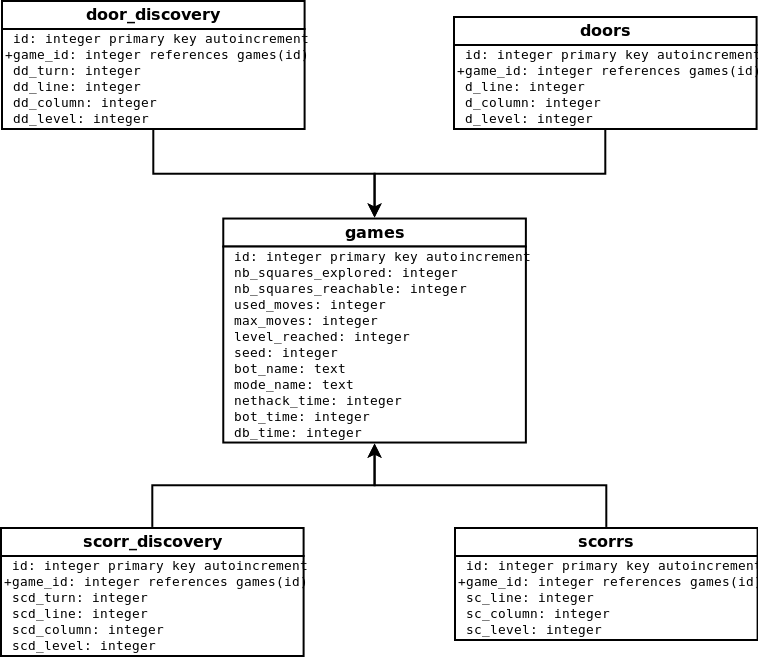
\includegraphics[width=\textwidth]{schema.png}}
	\caption{\label{fig:schema} Schéma de la base de données utilisée.}
\end{figure}
Une vue
fournissant certains détails supplémentaires \footnote{Nombre de portes
secrètes, nombre de portes secrètes trouvées, nombre de couloirs secrets et
nombre de couloirs secrets trouvés.} est aussi disponible afin de faciliter
l'utilisation de la base de données.
\\
Nous avons choisi d'utiliser une base de données {\em sqlite3}, celle-ci étant
assez simple à interfacer avec du {\em c}, mais aussi à interroger directement
par ligne de commande. Le grand avantage pour notre situation est aussi que les
bases de données {\em sqlite3} se présentent sous la forme d'un unique fichier,
celui-ci n'étant pas trop volumineux, il était parfaitement concevable de nous
échanger les bases de données de manière simple.
%TODO Parler des .def etc?


\subsubsection{Scripts de génération de graphiques}

Afin de visualiser les performances des différents bots, de pouvoir les comparer
facilement et de pouvoir vérifier statistiquement des propriétés de nethack,
nous avons mis en place des scripts permettant de générer de façon automatique
différents graphiques à partir d'une base de données. Ces graphiques se séparent
en trois catégories principales :
\begin{itemize}
\item Les graphiques permettant de mieux évaluer la répartition des performances
  des bots. Ceux-ci permettant entre autre de détecter que le bot ne fonctionne
  pas comme souhaité.
\item Les graphiques permettant de comparer les bots entre eux. Ceux-ci
  représentent la performance des bots sur un critère particulier en fonction du
  nombre maximal de mouvements autorisés. Ils permettent de départager les
  différentes stratégies par rapport à des objectifs.
\item Les graphiques analysant des données qui ne sont pas spécifiques au bot
  afin de permettre de vérifier certaines propriétés ou d'observer la
  distribution de certains événements aléatoires propres à nethack.
\end{itemize}
Tous les graphiques sont générés à l'aide de {\em gnuplot}, le type de sortie
peut facilement être modifié et permet ainsi de convenir à ce qui est attendu

\paragraph{Graphiques analysant un bot}

\subparagraph{Exemple}
Nous avons écrit un script permettant de générer un grand nombre de graphiques
indiquant la répartition des performances du bot. Celui-ci génère un graphique
par triplet
$\{\text{Bot},\text{Nb mouvements autorisés},\text{Caractéristique} \}$, il
faut par conséquent faire attention car suivant la base de données utilisée,
le temps de génération peut être conséquent. Voici un exemple d'un des graphes
produits par ce script.

\begin{figure}[H]
  \center{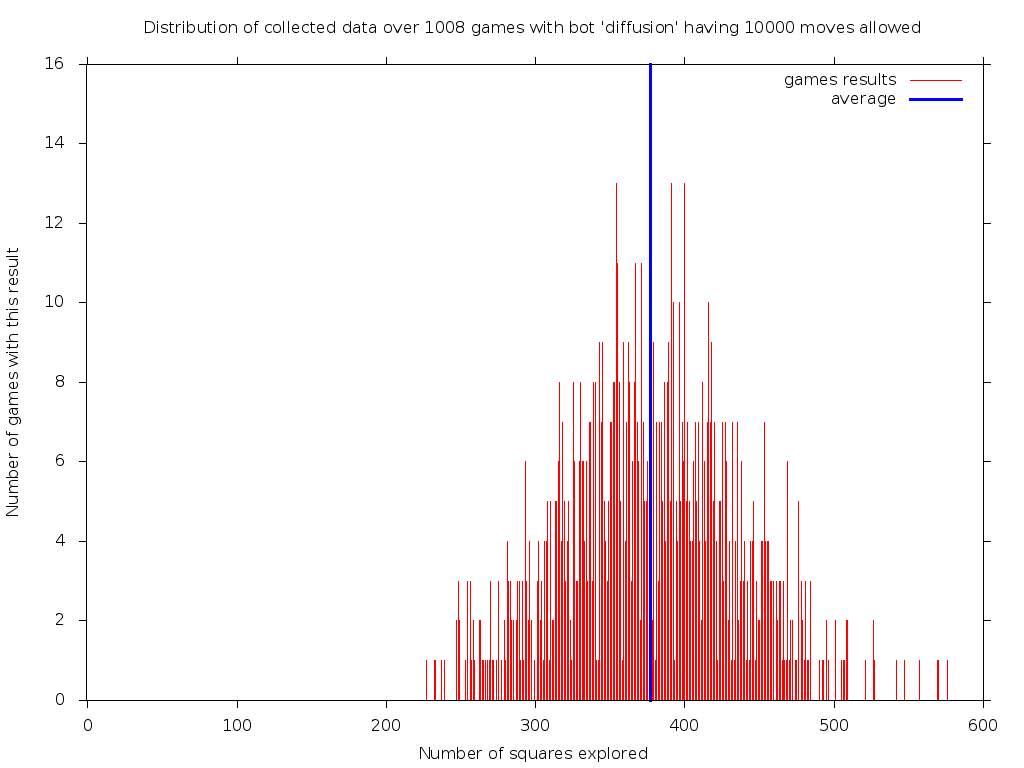
\includegraphics[width=\textwidth]{m_10000_nb_squares_explored.png}}
	\caption{\label{fig:impulse_graph} Un exemple de graphique montrant la
    répartition des performances}
\end{figure}

\subparagraph{Observation de caractéristiques du jeu}
Il est important de noter que ce script ne génère pas des graphes de répartition
que pour les performances du bot, il génère un graph similaire pour le résultat
maximal de chaque caractéristique, ce qui permet aussi d'observer la répartition
de celle-ci pour nethack. Nous avons ainsi constaté que la plupart des
caractéristiques \footnote{Nombre de portes secrètes présentes sur un niveau,
nombre de couloirs secrets présents sur un niveau et nombre de cases
explorables} que nous avons observées suivaient une distribution ayant en tout
cas l'apparence d'une gaussienne.
\\
Suivant les objectifs du bot, on peut donc imaginer qu'un bot se serve des
résultats obtenus afin de déterminer s'il est probable qu'il existe une autre
salle cachée où s'il a déjà tout visité. Cet aspect sera approfondi dans la
section {\em Analyses}.

\subparagraph{Observation de caractéristiques du bot}
Si l'exemple donné ci-dessus présente le nombre de cases explorées par le bot
comme suivant une gaussienne, certains aspects de répartition peuvent donner
plus d'informations, comme c'est le cas sur ce graphique.

\begin{figure}[H]
  \center{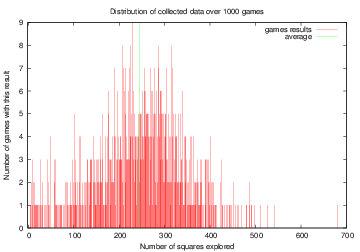
\includegraphics[width=0.5\textwidth]{nb_squares_explored.png}}
  \caption{\label{fig:nb_squares_explored} Un exemple de graphique montrant un
  dysfonctionnement du bot.}
\end{figure}

Le fait que la répartition des résultats ne suit pas une gaussienne n'est pas
forcément flagrant, en revanche, on distingue un nombre non négligeable de
parties ayant un nombre de cases explorées inférieur à 50, ce qui est très
faible en comparaison de la moyenne. En observant plus en détail une des
parties ayant obtenu un tel résultat, nous nous sommes rendus compte que le
problème venait du fait que les portes ne s'ouvraient plus, ce qui était dû à
une légère erreur lors d'une modification du noyau. Ces graphiques peuvent
donc aussi servir à détecter des dysfonctionnements lors de modifications du
noyau.

\paragraph{Graphiques comparant des bots}
Afin de comparer les performances des bots dans différents domaines, nous
avons écrit un script générant des graphiques permettant de visualiser
facilement les différences de résultats entre les différents bots. Celui-ci
génère un graphe par caractéristique observée, permettant ainsi de réduire le
nombre de manipulations à effectuer.

\begin{figure}[H]
  \center{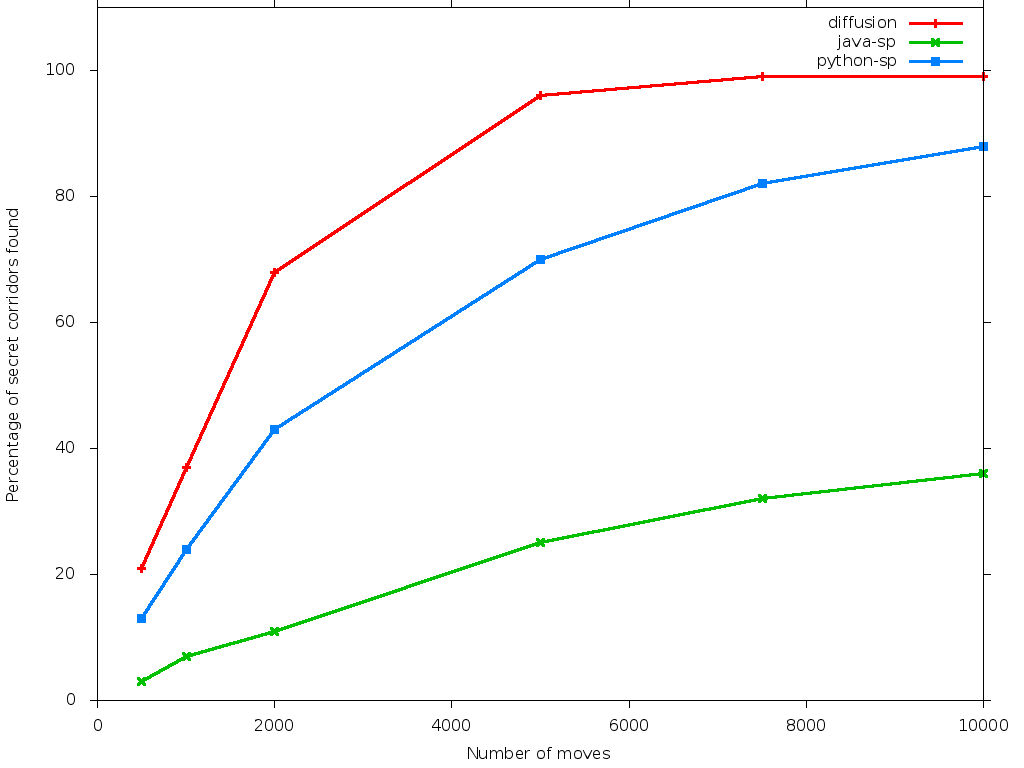
\includegraphics[width=\textwidth]{graph_percent_scorrs_found.png}}
  \caption{\label{fig:move_graph} Un exemple de graphique comparant des bots}
\end{figure}

Il est possible de donner des noms différents au même bot au fur et à mesure
qu'il évolue, en ajoutant des données à la même base, ainsi il est possible de
mesurer l'amélioration des performances. Ce raisonnement s'applique aussi à
des modifications de paramètres sur le bot diffusion par exemple, ce qui
pourrait permettre par exemple de faire de l'apprentissage sur les différents
paramètres afin de trouver les valeurs idéales. Le problème du bot diffusion
étant que lancer de nombreuses parties demande un temps d'exécution important.

\paragraph{Graphiques analysant la distribution des portes et couloirs secrets}
Afin d'observer des informations sur la distribution des portes et couloirs
secrets, nous avons créé des scripts permettant de visualiser le nombre de
portes secrètes ou de couloir secrets pour chaque emplacement. La possibilité de
visualiser l'information en deux ou en trois dimensions est fournie. En deux
dimensions, deux graphiques sont disponibles, l'un représentant le nombre
d'éléments trouvés en fonction de la ligne, l'autre en fonction de la colonne.
Seul le graphique en trois dimensions permet de visualiser les deux
simultanément. S'appuyant sur {\em gnuplot}, les scripts générant les graphiques
en trois dimensions proposent un mode interactif permettant de changer l'angle
de vue.

\begin{figure}[H]
  \center{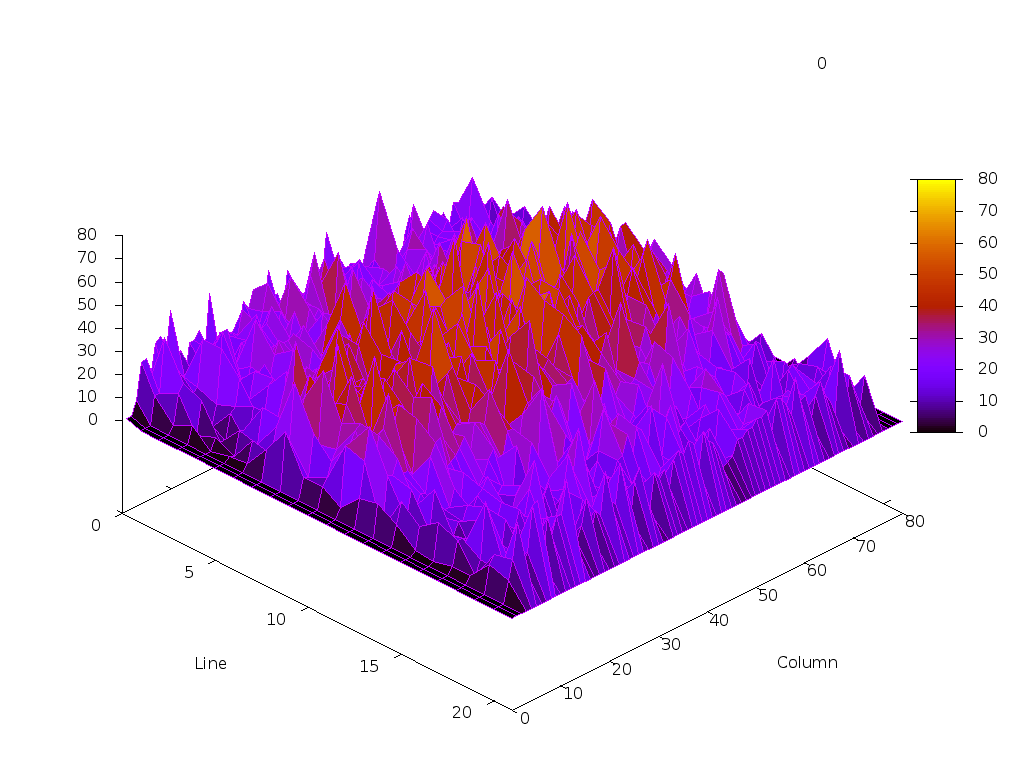
\includegraphics[width=\textwidth]{3d_exemple.png}}
  \caption{\label{fig:move_graph} Aperçu de la visualisation du nombre de
    couloirs secrets en fonction de la position.}
\end{figure}

L'utilité de ce type de graphiques sera approfondie dans la partie
{\em Analyses}.


\section{Analyses}

graphes, sous-section pour chaque "mode". Reprendre étude pièce rectangulaire.


\section{Problème simplifié : sortie d'une salle}

Afin d'étudier le problème de la recherche des portes secrètes de façon plus
théorique, nous avons réduit le nombre de paramètres aléatoires et simplifié
volontairement la situation.
\\
Dans ce niveau particulier :
\begin{itemize}
\item Le personnage apparaît au milieu d'une salle de $10$ lignes par $10$
  colonnes.
\item La salle est entourée de murs et un seul de ceux-ci contient une porte
  secrète.
  \footnote{Il y a {\em exactement} une porte secrète}
\item Tous les emplacements ont la même probabilité de contenir la porte
  secrète.
  \footnote{Ce point a été vérifié par l'expérience en générant un grand nombre
    de parties et en observant la répartition des portes secrètes}
\item Effectuer une recherche dans une des cases adjacentes au mur contenant la
  porte secrète a une probabilité de révéler celle-ci de $\frac{1}{7}$.
\item Le personnage est placé aléatoirement dans la pièce.
\end{itemize}

Voici un aperçu de l'apparence de la pièce, les carrés violets étant ceux où la
porte secrète peut se trouver.

\begin{center}
  \begin{tikzpicture}[scale=.5]
    % Drawing Walls part
    \foreach \x in {1,...,10}{
      \draw [fill=violet] (\x,  0) rectangle (\x + 1,  1);
      \draw [fill=violet] (\x, 11) rectangle (\x + 1, 12);
    }
    \foreach \y in {1,...,10}{
      \draw [fill=violet] ( 0, \y) rectangle ( 1, \y + 1);
      \draw [fill=violet] (11, \y) rectangle (12, \y + 1);
    }
    % Drawing internal grid
    \foreach \x in {1,...,10}{
      \foreach \y in {1,...,10}{
        \draw (\x,\y) rectangle (\x + 1,\y + 1);
      }
    }
  \end{tikzpicture}
\end{center}

Être certain d'avoir la meilleure stratégie étant trop complexe à nos yeux, nous
avons décider de chercher plutôt à définir une borne inférieure. Une fois
celle-ci obtenue, il est donc possible de la comparer aux résultats obtenus par
les bots. La différence entre ces deux résultats pourra être réduite de deux
façons :
\begin{itemize}
\item En augmentant la borne inférieure par des résultats théoriques.
\item En diminuant la borne supérieure par des modifications du bot.
\end{itemize}

\subsection{Approche théorique}

\subsubsection{Dominer la pièce}
Il est possible de fixer certaines cases où les recherches seront effectuées en
cherchant à minimiser ce nombre de cases, tout en ayant à portée tous les murs.
\footnote{Cette notion est comparable à la domination en théorie des graphes,
  les différences principales étant que l'on ne peut pas choisir n'importe quel
  sommet, certains sommets étant interdits et qu'il n'est pas nécessaire de
  dominer tous les sommets, mais uniquement les interdits.}
\\
En colorant en orange les cases où les recherches seront effectuées, et en
indiquant la portée des recherches par les carrés oranges transparents, le
résultat obtenu est le suivant :

\begin{center}
  \begin{tikzpicture}[scale=.5]
    % Drawing Walls part
    \foreach \x in {1,...,10}{
      \draw [fill=violet] (\x,  0) rectangle (\x + 1,  1);
      \draw [fill=violet] (\x, 11) rectangle (\x + 1, 12);
    }
    \foreach \y in {1,...,10}{
      \draw [fill=violet] ( 0, \y) rectangle ( 1, \y + 1);
      \draw [fill=violet] (11, \y) rectangle (12, \y + 1);
    }
    % Drawing internal grid
    \foreach \x in {1,...,10}{
      \foreach \y in {1,...,10}{
        \draw (\x,\y) rectangle (\x + 1,\y + 1);
      }
    }
    % Coloring squares and ranges of research
    \foreach \x in {1,4,7,10}{
      \draw [fill=orange] (\x,  1) rectangle (\x + 1,  2);
      \draw [fill=orange] (\x, 10) rectangle (\x + 1, 11);
      \draw [ultra thick, orange] (\x - 0.5, 0.5) rectangle (\x + 1.5,  2.5);
      \draw [ultra thick, orange] (\x - 0.5, 9.5) rectangle (\x + 1.5, 11.5);
    }
    \foreach \y in {1,4,7,10}{
      \draw [fill=orange] ( 1, \y) rectangle ( 2, \y + 1);
      \draw [fill=orange] (10, \y) rectangle (11, \y + 1);
      \draw [ultra thick, orange] (0.5, \y - 0.5) rectangle ( 2.5, \y + 1.5);
      \draw [ultra thick, orange] (9.5, \y - 0.5) rectangle (11.5, \y + 1.5);
    }
  \end{tikzpicture}
\end{center}
Il est assez évident qu'il est impossible de recouvrir chaque cases contenant
potentiellement une porte avec moins de carrés, car tous les coins\footnote{Ce
sont eux qui sont a portées du plus grand nombre de sommets à dominer.} sont
utilisés et aucune case n'est à portée de deux emplacements de recherches.

\subsubsection{Évolution des probabilités}
Si l'on ignore le coût des déplacements, prenant en compte uniquement les coûts
de recherche, le meilleur comportement semble être de commencer par chercher
dans les coins et d'utiliser ensuite les autres emplacements, ceci en
considérant qu'ils ont tous le même nombre de recherche au début. Il n'est en
revanche pas évident de déterminer si un coin sur lequel $n+1$ recherches ont
été effectuées a une chance plus élevée d'être à proximité d'une porte secrète
qu'un bord où $n$ recherches ont été effectuées.
\\
La probabilité initiale de découvrir une porte est égale à 
$\frac{1}{40} \times \frac{1}{7}$, la probabilité initiale de trouver une porte
secrète dans un coin est donc de : $4 \times \frac{1}{40} \times \frac{1}{7}$.
Lorsque des recherches sont effectuées, la partie représentant la probabilité de
trouver la porte secrète en sachant que l'on a cherché au bon endroit ne sera
pas modifiée ($\frac{1}{7}$). En revanche, la probabilité que la porte secrète
soit sur une case spécifique dépendra du nombre et de l'emplacement des
recherches déjà effectuées\footnote{Ce problème est semblable au fameux
problème de Mounty Hall, le point clé étant que l'on {\em sait} qu'il y a 
{\em exactement} une porte secrète parmi les 40 cases de murs}. Une intuition de
ce fait peut être donnée par l'exemple suivant : 10'000 recherches ont été
effectuées sur chacun des emplacements de recherches excepté sur celui se
situant en haut à gauche où aucune recherche n'a été effectuée, la probabilité
qu'une recherche sur cette case aboutissent est clairement de plus de 
$\frac{1}{10}$.
\\
Afin de présenter une preuve de cette différence de probabilité, nous allons
simplifier ce problème en considérant qu'il existe uniquement deux emplacements
où la porte secrète peut se trouver et que chaque recherche ne peut être à
portée que d'un seul d'entre eux.\\
On considère les notations suivantes :
\begin{itemize}
\item $Pos(P)$ est la position de la porte.
\item $T$ signifie que la porte a été trouvée.
\item $PT$ signifie que la porte n'a pas été trouvée.
\end{itemize}
Après une recherche en position $1$, on obtient l'arbre de probabilité suivant:

% Set the overall layout of the tree
\tikzstyle{level 1}=[level distance=3.5cm, sibling distance=3.5cm]
\tikzstyle{level 2}=[level distance=3.5cm, sibling distance=2cm]

% Define styles for bags and leafs
\tikzstyle{bag} = [text width=4em, text centered]
\tikzstyle{end} = [circle, minimum width=3pt,fill, inner sep=0pt]
\begin{center}
  \begin{tikzpicture}[grow=right, sloped]
    \node[bag] {Overall}
    child {
      node[bag] {Porte en $1$}        
      child {
        node[end] {}
        edge from parent
        node[above] {$T$}
        node[below]  {$\frac{1}{7}$}
      }
      child {
        node[end] {}
        edge from parent
        node[above] {$NT$}
        node[below]  {$\frac{6}{7}$}
      }
      edge from parent 
      node[above] {$Pos(P) = 1$}
      node[below]  {$\frac{1}{2}$}
    }
    child {
      node[bag] {Porte en $2$}
      child {
        node[end] {}
        edge from parent
        node[above] {$NT$}
        node[below]  {$1$}
      }
      edge from parent         
      node[above] {$Pos(P) = 2$}
      node[below]  {$\frac{1}{2}$}
    };
  \end{tikzpicture}
\end{center}

Si la première recherche a terminée sans que la porte n'ait été trouvée, les
nouvelles probabilités peuvent être aisément calculées :
\begin{itemize}
\item $P(Pos(P) = 1) = \frac{\frac{1}{2} \times \frac{6}{7}}
                            {\frac{1}{2} \times \frac{6}{7} +
                             \frac{1}{2}}
                     = \frac{6}{13}$
\item $P(Pos(P) = 2) = \frac{\frac{1}{2}}
                            {\frac{1}{2} \times \frac{6}{7} +
                             \frac{1}{2}}
                     = \frac{7}{13}$
\end{itemize}

\subsubsection{Calcul de la probabilité}
Nous avons déjà démontré que deux emplacements ne sont plus équiprobables si
plus de recherches ont été effectués sur l'un que sur l'autre. Il est aussi
évident que la méthode présentée ci-dessus sera très difficile à appliquer sur
un grand nombre de recherches. C'est pour cette raison que nous avons développé
une autre approche, permettant de calculer les probabilités de façon plus simple
et aussi beaucoup plus rapide pour un ordinateur.\\
À partir de l'arbre de probabilité présentés précédemment, il est facile de voir
que la probabilité qu'une recherche soit fructueuse dépend uniquement de la
probabilité qu'une porte cachée se situe à portée de l'endroit où est effectuée
la recherche.
\\
Afin de résoudre ce problème dans un cas plus général, nous définissons
certaines notations :
\begin{itemize}
\item $W$ est l'ensemble des emplacements de recherches.
  $W = \{W_0,W_1, ... , W_{|W| -1} \}$
\item $R(W_k)$ représente le nombre de recherche faîtes sur l'emplacement $W_k$.
\item $V(W_k)$ représente le nombre de voisins de l'emplacement $W_k$
  susceptibles de contenir une porte secrètes.
\item $P(W_k = V)$ représente la probabilité que la porte secrète soit voisine
  de l'emplacement $W_k$.
\item $p$ est la probabilité de trouver une porte sachant qu'un de ses voisins
  contient la porte secrète.\footnote{$\frac{1}{7}$ dans le cas étudié ici.}
\end{itemize}

En accord avec les règles de probabilités, on définit donc la probabilité
qu'une recherche aboutisse ainsi :
$$P(W_k = V) = \frac{\text{cas favorables}(W_k)}{\text{cas possibles}}$$
Ces deux éléments peuvent être définis ainsi :
\begin{itemize}
\item $\text{cas favorables}(W_k) = V(W_k) * (1-p)^{R(W_k)}$
\item $\text{cas possibles} = \sum\limits_{k=0}^{|W| - 1}{V(W_k) * (1-p)^{R(W_k)}}$
\end{itemize}

On aboutit donc à la formule suivante pour définir la probabilité que la porte
soit à portée de l'emplacement $W_k$:
$$ P(W_k = V) = \frac{V(W_k) *(1-p)^{R_k}}{\sum\limits_{k=0}^{|W| - 1}{V(W_k) * (1-p) ^{R_k}}}$$
Comme $\text{cas possibles}$ n'est pas fonction de $k$, il est possible de
comparer l'intérêt de différentes cases uniquement en comparant les valeurs de
$\text{cas favorables}(W_k)$.
\\
Dans notre situation:
\begin{itemize}
\item Pour les coins, $V(W_k) = 4$.
\item Pour les bords, $V(W_k) = 3$.
\end{itemize}
Soient $k_1$ et $k_2$ tels que:
\begin{itemize}
\item $W_{k_1}$ est un coin.
\item $W_{k_2}$ est un bord.
\item $R(W_{k_1}) - R(W_{k_2}) = i$ avec $(1-p)^i = \frac{3}{4}$ ce qui implique
  que $i = \frac{\log(\frac{3}{4})}{\log(1-p)}$.\footnote{$i = 1,866$ dans notre
    cas.}
\end{itemize}
On obtient
$$\begin{array}{l c l}
\text{cas favorables}(W_{k_1})
&= &V(W_{k_1}) * (1-p)^{R(W_{k_1})}\\
&= &4 * (1-p)^{R(W_{k_2}) + i}\\
&= &4 * (1-p)^{R(W_{k_2})} * (1-p)^i\\
&= &4 * (1-p)^{R(W_{k_2})} * \frac{3}{4}\\
&= &3 * (1-p)^{R(W_{k_2})}\\
&= &V(W_{k_2}) * (1-p)^{R(W_{k_2})}\\
&= &\text{cas favorables}(W_{k_2})
\end{array}$$
Une implication importante de ce résultat est que pour un nombre de recherches
$n$, l'idéal sera que chaque coin ait eu $i$ recherches de plus que chaque bord.
De plus, la valeur de ce $i$ dépendra uniquement de $p$.

\subsubsection{Minoration du nombre moyen de recherches}
Si l'on désire minimiser le nombre moyen de recherches\footnote{Sans prendre du
  tout en compte le nombre de déplacements nécessaires}, il faut toujours
rechercher à l'emplacement ayant la plus haute probabilité d'être proche d'une
porte secrète. En effet, les chances que la porte soit trouvée sont maximales
pour un nombre de recherches $k$ si l'on se trouve dans un cas où les différents
emplacements de recherches ont des probabilités aussi proches que possibles.
\\
Nous noterons :
\begin{itemize}
\item $P_k$ : La probabilité de trouver la porte secrète en $k$ recherches au
  maximum.
\item $R_k$ : La probabilité de trouver la porte secrète en exactement $k$
  recherches.
\item $P(door)$ : La probabilité que la porte soit à l'emplacement de la
  recherche, cet emplacement est choisi comme étant le plus probable au moment
  de la recherche. Cette probabilité est calculée à l'aide de la formule trouvée
  précédemment.
\item $p$ : La probabilité de trouver la porte sachant qu'elle est voisine de la
  case où la recherche a été effectuée.
\end{itemize}
On obtient donc :
$$P_{k+1} = P_k + (1 - P_k) * P(door) * p$$
$$R_{k+1} = P_{k+1} - P_{k}$$
Quelque soit la stratégie choisie, il est donc évident que le nombre moyen de
recherches sera supérieur ou égal à $\sum\limits_{k=0}^{\infty} k * R_k$.
\\
Nous avons minoré cette valeur à l'aide d'un programme faisant l'addition de ces
termes tant que $R_k > 10^{-10}$ et nous avons obtenu environ $77,75$.

\subsection{Comparaison des résultats expérimentaux avec les valeurs théoriques}
La moyenne du nombre d'actions nécessaire au bot diffusion pour ouvrir la porte
sur 100 parties était de $158$, ce résultat est relativement proche de la borne
inférieure ($77,75$) si l'on prend en compte que la borne inférieure a été
calculée en ignorant totalement le coût des mouvements. En effet, afin
d'optimiser le nombre d'action moyen, le bot est obligé d'effectuer plusieurs
recherches sur un emplacement tandis que la stratégie utilisée pour calculer la
borne inférieure coûterait un nombre d'action très élevé en raison du nombre de
déplacements élevés qu'elle utilise.
\begin{figure}[H]
  \center{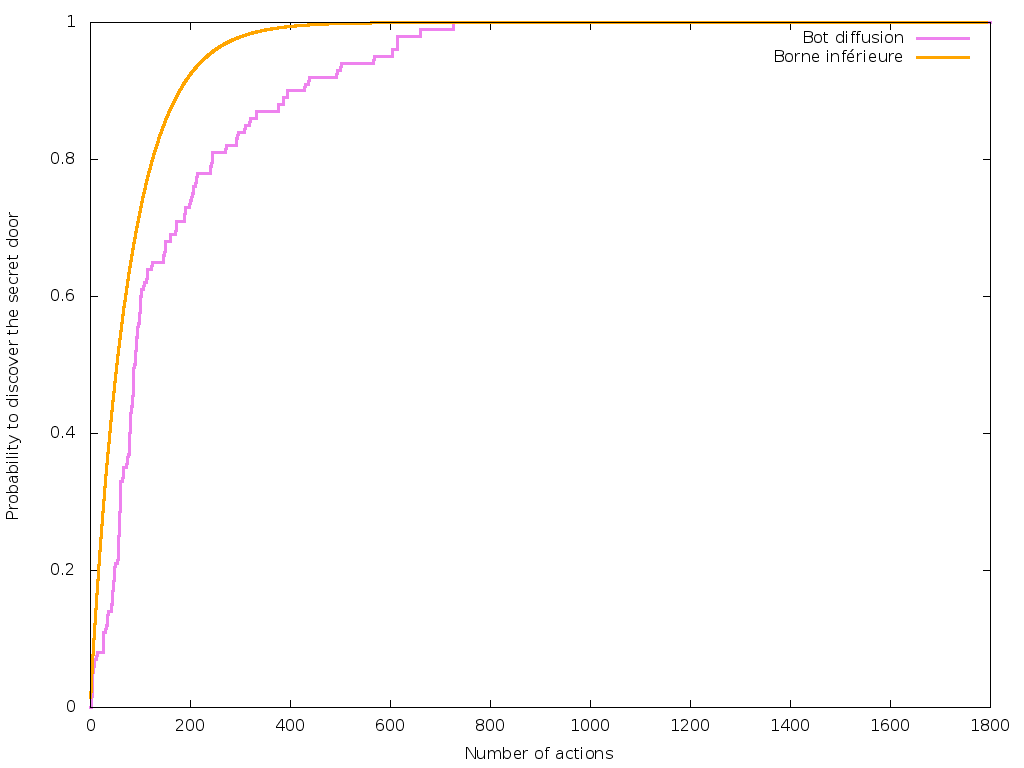
\includegraphics[width=\textwidth]{../images/compare.png}}
	\caption{\label{fig:compare} Graphique comparant les valeurs expérimentales du
  bot diffusion aux valeurs obtenues.}
\end{figure}

Une possibilité d'augmenter la borne inférieure pourrait être de minorer le
nombre de mouvement moyen. En effet, si l'on ignore totalement le coût des
recherches, il reste tout de même un nombre de mouvement non négligeable à
effectuer afin d'arriver à portée de la porte secrète (dont on ignore la
position).

\section{Documentation}
Utilisation de Doxygen, manuel d'utilisation, nombreux README, commentaires de
code (hors Doxygen), etc.

\section{Tests}
Quelques tests unitaires, tests via dummy client, tests du genre "je lance, ça
plante pas", tests avec les bots, etc.

\subsection*{Repérage des problèmes}
Utilisation du viewer pour comprendre ce qui ne va pas, utilisation de gdb,
quelques tentatives infructueuses de test de couverture (gcov), de profilage
(gprof) et mémoire (valgrind).

\section{Travail en équipe, organisation}

Utilisation de git.
Comparer avec le travail en plus grande équipe.

\subsection{Conventions}
Commentaires en anglais, respect des conventions employées par les
développeurs de NetHack lors des modifications du code source du jeu,
utilisations des espaces vs tab, convention de nommage, positionnement des
accolades, etc.

\section{Améliorations possibles}

\section{Conclusion}

\end{document}
